\documentclass[%
 aip,
% jmp,
% bmf,
% sd,
% rsi,
 amsmath,amssymb,
%preprint,%
 reprint,%
%author-year,%
%author-numerical,%
% Conference Proceedings
]{revtex4-1}

\usepackage{graphicx}% Include figure files
\usepackage{dcolumn}% Align table columns on decimal point
\usepackage{bm}% bold math
%\usepackage[mathlines]{lineno}% Enable numbering of text and display math
%\linenumbers\relax % Commence numbering lines

\usepackage[utf8]{inputenc}
\usepackage[T1]{fontenc}
\usepackage{mathptmx}
\usepackage{etoolbox}
\usepackage{hyperref}
\usepackage{float}
\usepackage{svg}

% \usepackage{unicode-math}
% \setmathfont{Latin Modern Math}

\newenvironment{proof}{\noindent\textbf{Proof.}}{\hfill $\square$\par}
\hypersetup{
    colorlinks=true,
    linkcolor=blue,
    urlcolor=blue,
    citecolor=blue,
    linkbordercolor=white
}

%% Apr 2021: AIP requests that the corresponding 
%% email to be moved after the affiliations
\makeatletter
\def\@email#1#2{%
 \endgroup
 \patchcmd{\titleblock@produce}
  {\frontmatter@RRAPformat}
  {\frontmatter@RRAPformat{\produce@RRAP{*#1\href{mailto:#2}{#2}}}\frontmatter@RRAPformat}
  {}{}
}%
\makeatother
\begin{document}

\preprint{AIP/123-QED}

\title[Swarming dynamics under different orientation (chiral) coupling mechanisms]{Swarming dynamics under different orientation (chiral) coupling mechanisms\\ \;}
% Force line breaks with \\
\author{A. Author}
 \altaffiliation[Also at ]{Physics Department, XYZ University.}%Lines break automatically or can be forced with \\
\author{B. Author}%
 \email{Second.Author@institution.edu.}
\affiliation{ 
Authors' institution and/or address%\\This line break forced with \textbackslash\textbackslash
}%

\author{C. Author}
 \homepage{http://www.Second.institution.edu/~Charlie.Author.}
\affiliation{%
Second institution and/or address%\\This line break forced% with \\
}%

\date{\today}% It is always \today, today,
             %  but any date may be explicitly specified

\begin{abstract}
    abstract abstract abstract abstract abstract abstract abstract abstract abstract abstract abstract abstract abstract abstract abstract abstract abstract abstract abstract abstract abstract abstract abstract abstract abstract abstract abstract abstract abstract abstract abstract abstract abstract abstract abstract abstract abstract abstract abstract abstract abstract abstract abstract abstract abstract abstract abstract abstract abstract abstract abstract abstract abstract abstract abstract abstract abstract abstract abstract abstract abstract abstract abstract abstract abstract abstract abstract abstract abstract abstract abstract abstract abstract abstract abstract abstract abstract abstract abstract abstract abstract abstract abstract abstract abstract abstract abstract abstract abstract abstract abstract abstract abstract abstract abstract abstract 
\end{abstract}

\maketitle

% \begin{quotation}
%     The ``lead paragraph'' is encapsulated with the \LaTeX\
%     %
%     The lead paragraph will only be found in an article being prepared for the journal \textit{XXX}.
% \end{quotation}

\section{INTRODUCTION\protect\\ }
% The line break was forced \lowercase{via} \textbackslash\textbackslash
Synchronization and swarming are two typical self-organization behaviors representing the intrinsic dynamial and spatial ordering of units in complex systems.
The study of self-organized coordination of intrinsic degrees of freedom/rhythms within complex systems has deepened our understanding of self-organization in complex systems, including various levels of synchronization, partial synchronization, extended states, and chimera states\cite{pikovsky2001universal,acebron2005kuramoto,rodrigues2016kuramoto,boccaletti2018synchronization,zou2021quenching,arenas2008synchronization}.
In terms of synchronization theory, at the micro level, various analysis methods have been established, such as the master stability function (MSF) \cite{pecora1998master}, which has played an important role in the study of multi-oscillator synchronization problems. At the statistical and macro levels, successful approaches include the self-consistent equation method by Kuramoto et al. \cite{kuramoto1984chemical}, the Watanabe-Strogatz transformation \cite{watanabe1994constants,strogatz1988simple}, and the Ott-Antonsen ansatz proposed by Ott and Antonsen \cite{ott2009long}.
Cluster behavior research focuses on the self-organized coordination of spatial movement in complex systems, contributing to our understanding of collective behavior. Spatial cluster behavior can emerge at different scales, such as animal clusters \cite{buhl2006disorder,niven2012honeybees,bazazi2008collective}, bacterial directed motion \cite{wioland2016directed,lushi2014fluid}, and other phenomena \cite{zhang2010collective,shi2010understanding,debnath2016communication}. Numerous studies based on diverse cluster models and extensive experimental investigations \cite{vicsek1995novel,farrell2012pattern,nagai2015collective,grossmann2014vortex,chepizhko2013optimal,sumino2012large,yan2016reconfiguring} have revealed various collective spatial interactions and patterns in complex systems.

The Kuramoto model\cite{kuramoto1975international} and the Vicsek model\cite{vicsek1995novel} are two well-known models that describe synchronization and swarming, respectively. The Kuramoto model describes the synchronization of oscillators with a phase variable, and the Vicsek model describes the alignment of self-propelled particles with a velocity variable. Both models have been widely studied and applied in various fields, such as physics \cite{pantaleone1998stability,wiesenfeld1996synchronization}, biology \cite{aihara2008mathematical,o2016dynamics,neda2000physics,majhi2019emergence}, and engineering\cite{motter2019author,strogatz2005crowd,rohden2012self}.
In recent years, there has been a notable surge in the research progress concerning the interplay between synchronization dynamics and cluster dynamics \cite{o2017oscillators,kruk2018self,levis2019activity,ceron2023diverse,ling2022spatial}, which has led to the development of models that combine the Kuramoto and Vicsek models. 

This paper continues this line of research by proposing a model that combines the Kuramoto and Vicsek models, aiming to undertake a more comprehensive exploration and integration of the interdisciplinary field encompassing synchronization dynamics and cluster dynamics. In Ceron et al.'s \cite{ceron2023diverse} and Levis et al.'s \cite{levis2019activity} studies, the behavior of oscillators which are non-identical (oscillators have different natural frequencies), chiral
(oscillators have inherent clockwise and counterclockwise circular orbits), and locally coupled (oscillators can only couple to motion and phase of neighbors within a given radius) was numerically investigated. Here, we introduce a model that combines these three characteristics and study the synchronization and cluster behaviors of it. We obtain the analytic solutions of the model and explore the phase diagram. 

The paper is organized as follows. In Section \ref{sec:model}, we introduce the model and the numerical methods used to study it. In Section \ref{sec:behavior}, we present the behavior of the model and discuss the states it exhibits. In Section \ref{sec:orderParam}, we introduce order parameters to distinguish the states and present the phase diagram of the model. In Section \ref{sec:analysis}, we derive the critical lines of the transitions between states and analytically explain diverse emergence behaviors driven by the model. Finally, in Section \ref{sec:conclusions}, we summarize the results and discuss the implications of the model.

\section{\label{sec:model} Model}

\begin{figure*}
    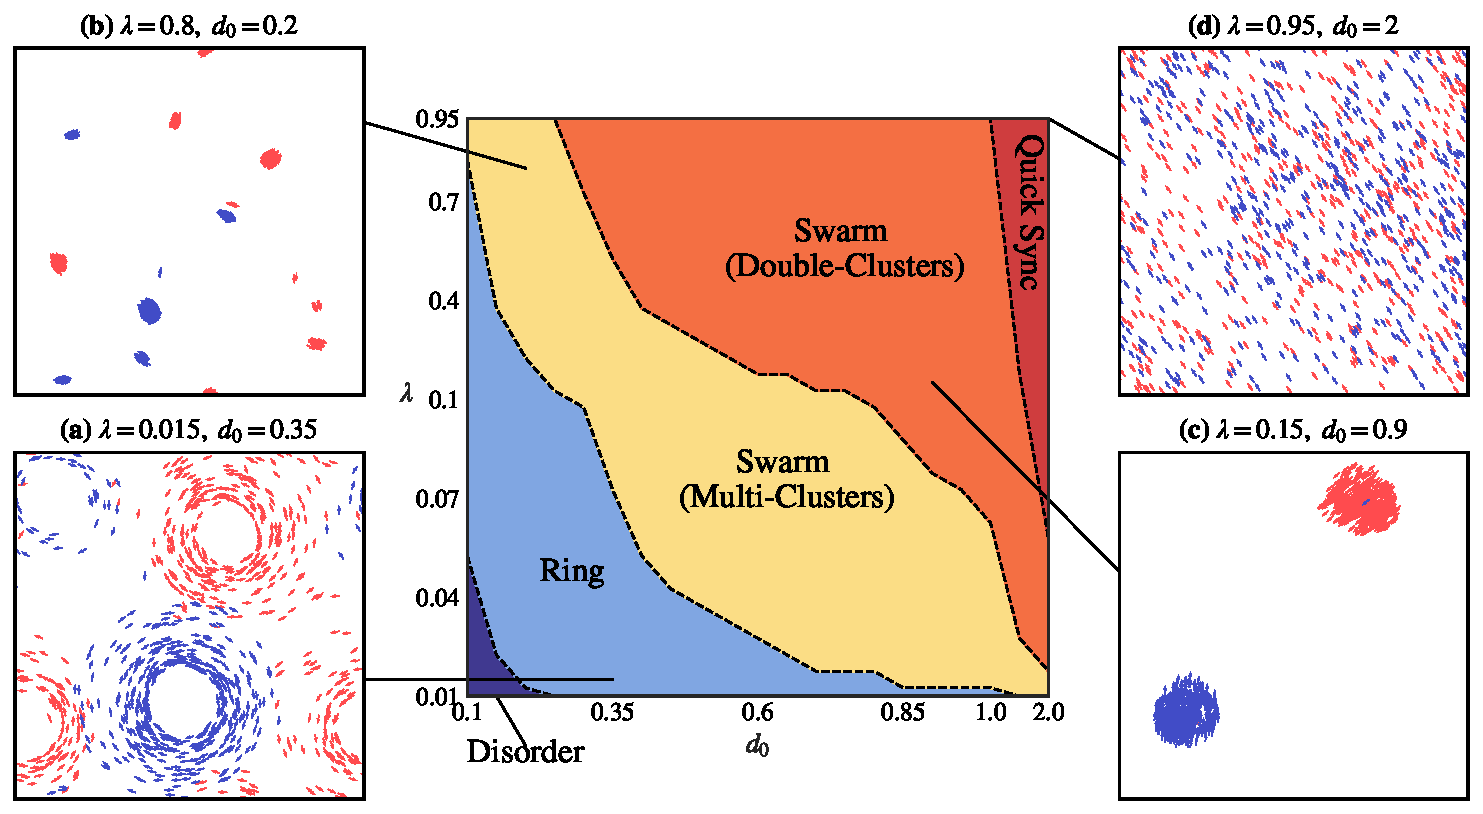
\includegraphics[width=\textwidth]{./figs/phaseDiagram.pdf}
    \caption{
        \label{fig:phaseDiagram} Phase diagram of model Eq.~(\ref{eq:dotxi})-(\ref{eq:dotthetai}) in the $(\lambda$-$d_0)$ plane. The boundaries between states are analytical approximations given by Subsection~\ref{critical}. 
        For the sake of clarity, the scale of $\lambda$ and $d_0$ is non-linear (For $\lambda$ in $\left[ 0.01, 0.1 \right]$ and $\left[ 0.1, 1 \right]$, step length is $0.1$ and $0.05$, respectively. For $d_0$ in $\left[ 0.1, 1 \right]$ and $\left[ 1, 2 \right]$, step length is $0.05$ and $0.5$, respectively).
        \textbf{(a)}, The snapshots of Ring ($\lambda=0.015,\ d_0=0.35$). 
        \textbf{(b)}, Swarm (Multi-Clusters) ($\lambda=0.4,\ d_0=0.3$).
        \textbf{(c)}, Swarm (Double-Clusters) ($\lambda=0.15,\ d_0=0.9$).
        \textbf{(d)}, Quick Sync ($\lambda=0.95,\ d_0=2$). Two types of chiral oscillators are represented by red ($\omega_i > 0$) and blue 
        ($\omega_i < 0$) arrows, respectively. 
    }
\end{figure*}

Oscillators have a spatial position $\mathbf{r}_i=\left( x_i, y_i \right)$ and an internal phase $\theta_i$ which evolve according to equations:

\begin{eqnarray}
    \dot{x}_i&=&v\cos \theta _i\;,\label{eq:dotxi}
  \\
    \dot{y}_i&=&v\sin \theta _i\;,\label{eq:dotyi}
  \\
    \dot{\theta}_i&=&\omega _i+\lambda \sum_{j=1}^N{A_{ij}\sin \left( \theta _j-\theta _i \right)}
    \label{eq:dotthetai}
\end{eqnarray}
for $i=1,2,\ldots,N$, where $N$ is the number of oscillators. As per Eq.~(\ref{eq:dotxi}) and (\ref{eq:dotyi}), each oscillator moves with a constant speed $v$ in the direction of its current phase $\theta_i$. The phase $\theta_i$ evolves according to Eq.~(\ref{eq:dotthetai}), where $\omega_i$ is the natural frequency of the $i$th oscillator, $\lambda$ is the coupling strength, and $A$ is the adjacency matrix of the network, with $A_{ij}=1$ if there is a connection from $i$th to $j$th oscillator, and $A_{ij}=0$ otherwise. We can consider Eq.~(\ref{eq:dotxi})-(\ref{eq:dotthetai}) as a generalization of the Kuramoto model and the Vicsek model in the sense that it includes both the phase and the spatial position of the oscillators.

Each oscillator $i$ is connected to all the oscillators within an
action radius $d_0$ of its position. The adjacency matrix $A$ is defined as:

\begin{equation}
    A_{ij}=\begin{cases}
        1,&		\left| \mathbf{r}_i-\mathbf{r}_j \right|\le d_0\\
        0,&		\left| \mathbf{r}_i-\mathbf{r}_j \right|>d_0\\
    \end{cases}
\end{equation}
where $\left| \mathbf{r}_i-\mathbf{r}_j \right|$ is the Euclidean distance between oscillators. 

For simplicity, we consider oscillators are initially distributed uniformly in a two-dimensional square with side length $L$ and periodic boundary conditions. Their positions $\mathbf{r}_i\left( t \right) =\left( x_i\left( t \right) ,y_i\left( t \right) \right) $ at given time $t$ are given by:

\begin{equation}
    \begin{array}{c}
        x_i\left( t+\Delta t \right) =x_i\left( t \right) +v\cos \theta _i\left( t \right) \Delta t\,\,\mathrm{mod}\ L,\\
        x_i\left( t+\Delta t \right) =x_i\left( t \right) +v\cos \theta _i\left( t \right) \Delta t\,\,\mathrm{mod}\ L,\\
    \end{array}
\end{equation}
where $\Delta t$ is the discrete time step. When two oscillators are on opposite sides of the square, the absolute value of the difference between one of their coordinates is greater than $L/2$. In this case, we take the minimum distance between them, which is the distance between the two points in the periodic boundary conditions. For a given pair of points $\mathbf{r}_i$ and $\mathbf{r}_j$, the distance between them is $\left| \mathbf{r}_i-\bar{\mathbf{r}}_j \right|$, where $\bar{\mathbf{r}}_j=\left( \bar{x}_j,\bar{y}_j \right)$ is the adjusted position of the $j$th oscillator, given by:
\begin{eqnarray}\label{eq:adj_pos1}
    \bar{x}_j=\begin{cases}
        x_j,&		\left| x_i-x_j \right|\le L/2\\
        x_j+L,&		x_i-x_j>L/2\\
        x_j-L,&		x_j-x_i>L/2\\
    \end{cases},
    \\
    \bar{y}_j=\begin{cases}\label{eq:adj_pos2}
        y_j,&		\left| y_i-y_j \right|\le L/2\\
        y_j+L,&		y_i-y_j>L/2\\
        y_j-L,&		y_j-y_i>L/2\\
    \end{cases}.
\end{eqnarray}
$\left| \mathbf{r}_i-\bar{\mathbf{r}}_j \right|$ can be proved to be the minimum distance between $\mathbf{r}_i$ and $\mathbf{r}_j$ in the periodic boundary conditions (see the proof in Appendix \ref{sec:adj_pos}).

Finally, we consider that the natural frequencies $\omega_i$ are distributed in two symmetric uniform distributions, representing two types of chirality. Exactly half of the oscillators have natural frequencies in the range $\left[ \omega _{\min},\omega _{\max} \right]$ ($\omega_i \sim U\left( \omega _{\min},\omega _{\max} \right), i=1,2,\ldots,N/2$) and the other half in the range $\left[ -\omega _{\max},-\omega _{\min} \right]$ ($\omega_i \sim U\left( -\omega _{\max},-\omega _{\min} \right), i=N/2+1,N/2+2,\ldots,N$).

\begin{figure*}
    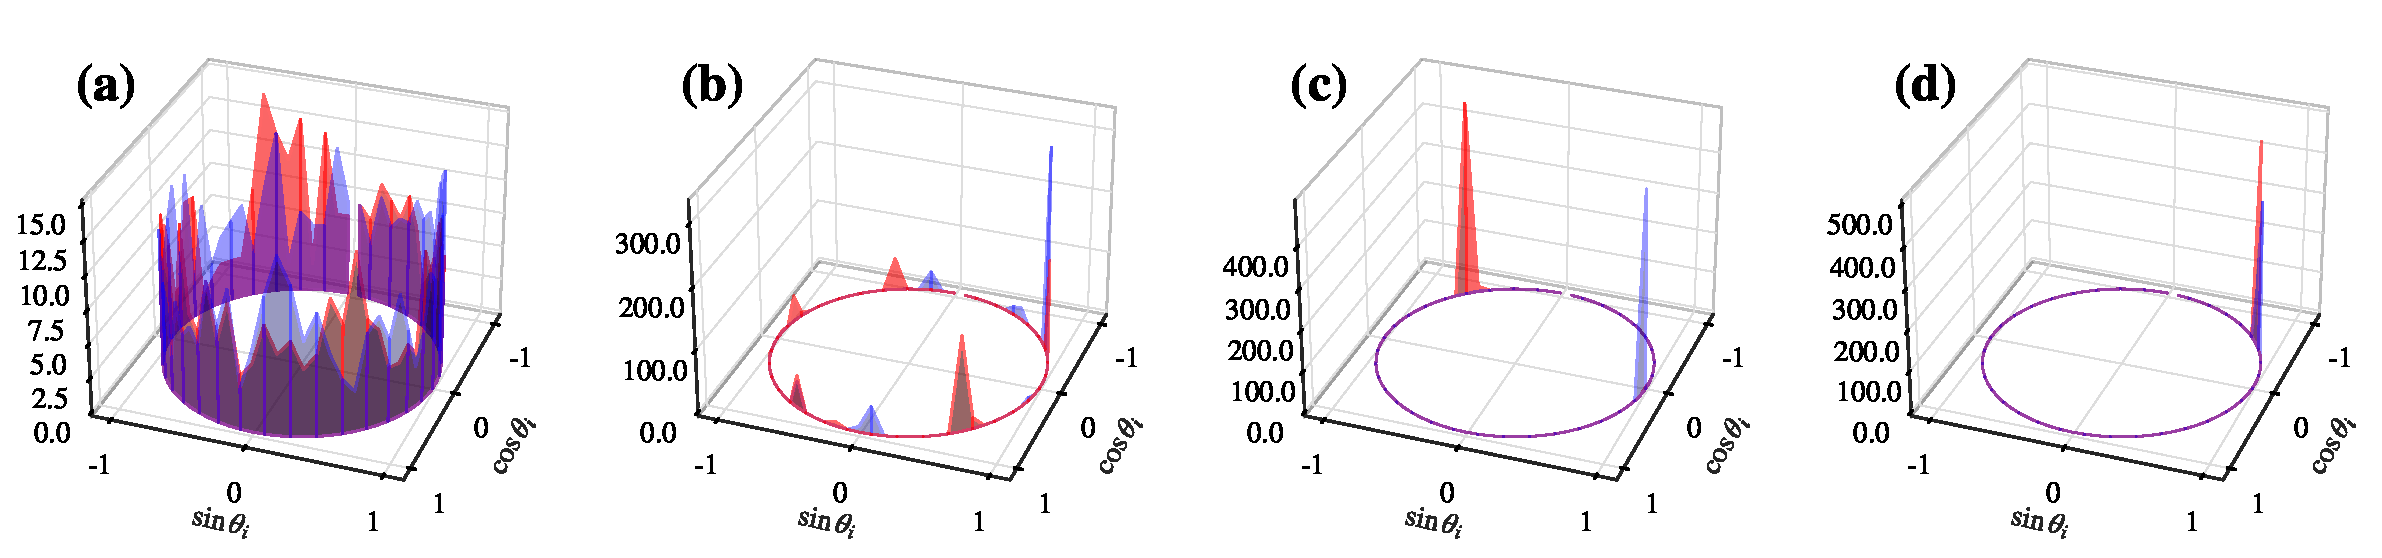
\includegraphics[width=\textwidth]{./figs/phaseHist.pdf}
    \caption{
        \label{fig:phaseHist} Histogram of the oscillators' phases.
        \textbf{(a)}, Ring state ($\lambda=0.015,\ d_0=0.35$).
        \textbf{(b)}, Swarm state (Multi-Clusters, $\lambda=0.8,\ d_0=0.2$).
        \textbf{(c)}, Swarm state (Double-Clusters, $\lambda=0.15,\ d_0=0.9$).
        \textbf{(d)}, Quick Sync state ($\lambda=0.95,\ d_0=2$). The histograms are calculated with $70$ bins.
    }
\end{figure*}

\begin{figure*}
    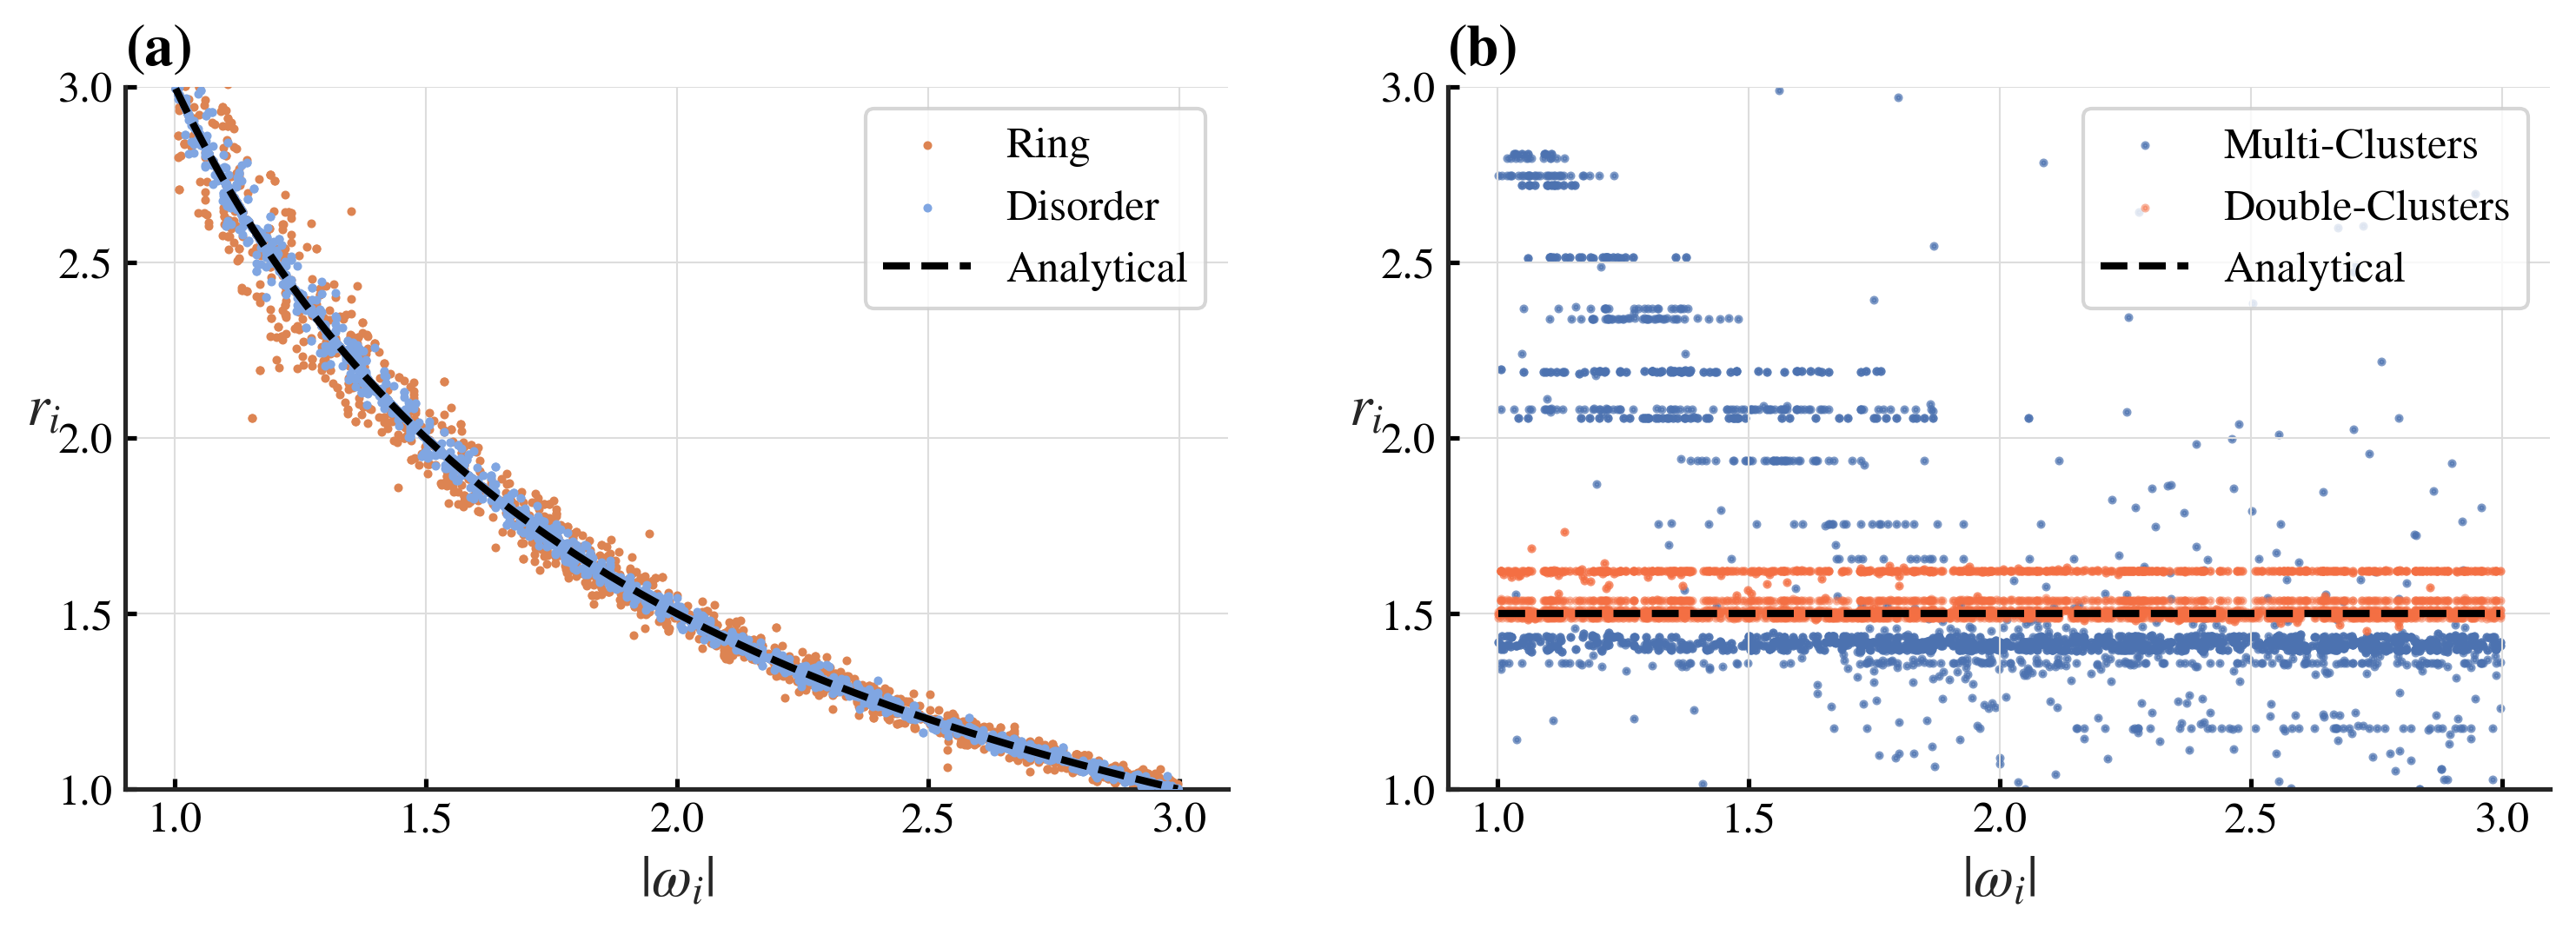
\includegraphics[width=\textwidth]{./figs/radiusOmega.png}
    \caption{
        \label{fig:radiusOmega} The real-time and analytical rotational radius.
        \textbf{(a)}, Radius for the Disorder ($d_0=0.1$, $\lambda=0.01:0.06$) and Ring ($d_0=0.1$, $\lambda=0.06:0.1$). The real-time rotational radius is almost constant and close to $v/\omega_i$ for each oscillator. 
        \textbf{(b)}, Radius for Swarm (Multi-Clusters, $d_0=0.15:0.25$, $\lambda=0.95$) and (Double-Clusters, $d_0=2$, $\lambda=0.02:0.05$). Analytical line is only for Double-Clusters.
        All the above simulations are calculated at $t=60000$. 
    }
\end{figure*}

\section{\label{sec:behavior}Behavior}

We performed numerical simulations of the model to probe the behavior of its solutions (see Appendix \ref{sec:numerics} for details on the numerical methods). 
$N=1000$ oscillators were distributed uniformly in the square of length $L=10$ and their natural frequencies were distributed in the range $\left[ \omega _{\min},\omega _{\max} \right]=\left[ 1,3 \right]$ and $\left[ -\omega _{\max},-\omega _{\min} \right]=\left[ -3,-1 \right]$.
Two-parameter of coupling strength $\lambda$ and action radius $d_0$ are presented in the phase diagram in Fig.~\ref{fig:phaseDiagram}. We found the system settles into five states: \textbf{Disorder}, \textbf{Ring}, \textbf{Swarm} (which can be further divided into \textbf{Multi-Clusters} and \textbf{Double-Clusters}), and \textbf{Quick Sync}. In Fig.~\ref{fig:phaseDiagram} we show the snapshots of the last three states and where these states are located in the phase diagram. The Disorder state is shown in Fig.~\ref{fig:disorderState}a.
We next discuss these five states.

\begin{figure}[b]
    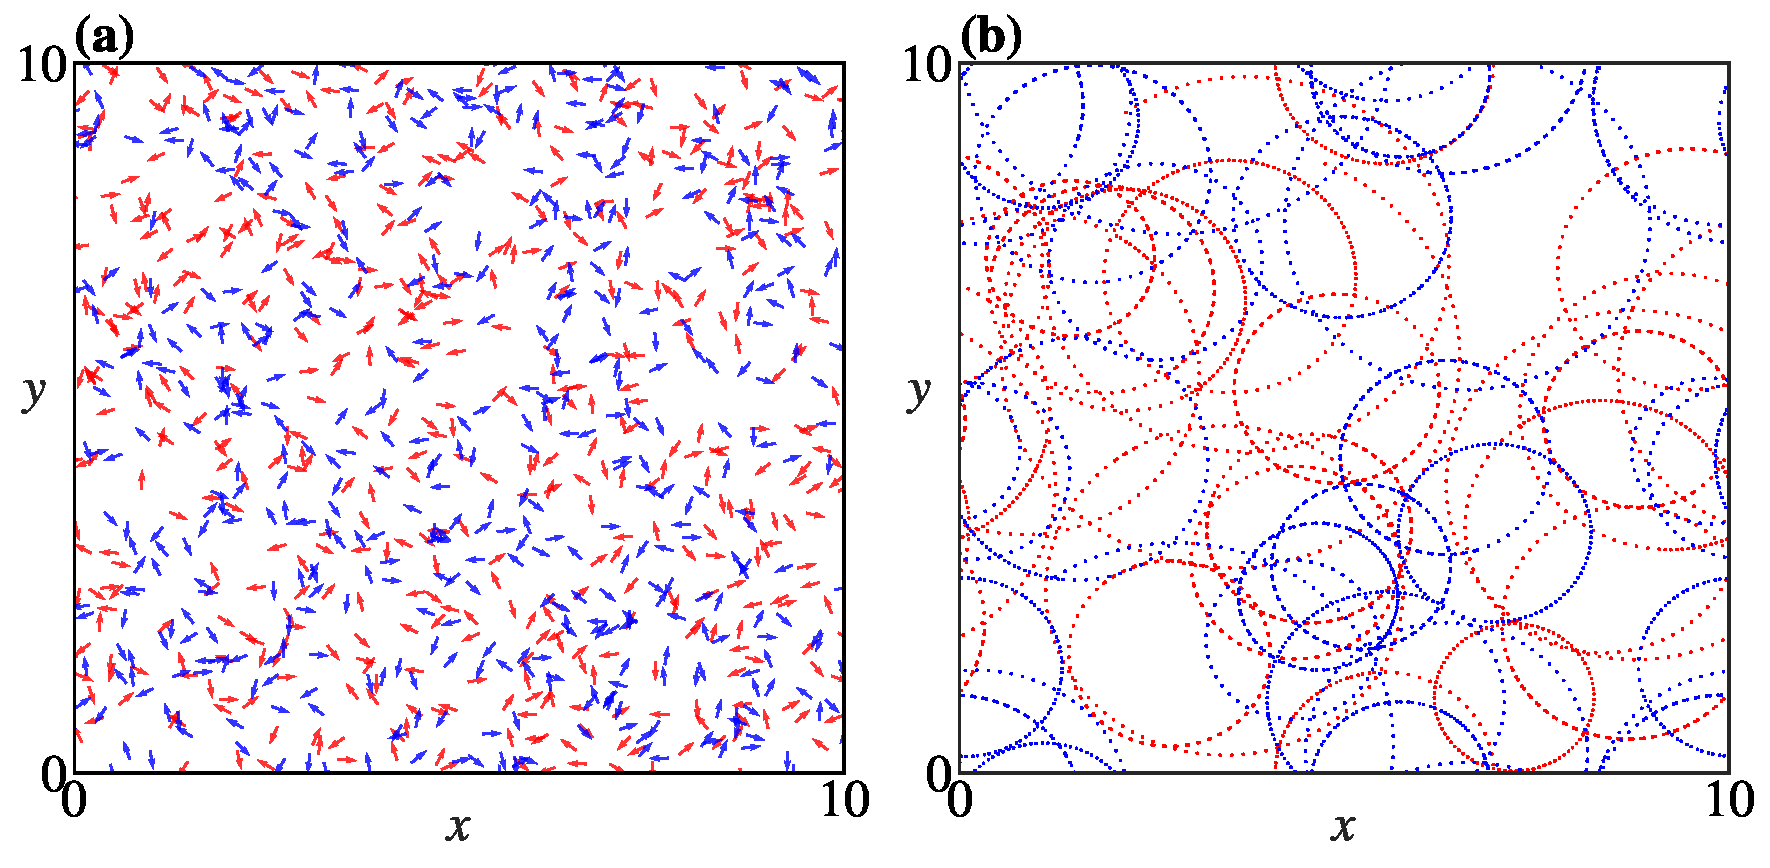
\includegraphics[width=0.48\textwidth]{./figs/disorderState.pdf}
    \caption{
        \label{fig:disorderState} Key properties of the Disorder state. 
        \textbf{(a)}, The snapshot of the Disorder state ($\lambda=0.01,\ d_0=0.1, T=60000$). 
        \textbf{(b)}, The scatter plot of last 100 time steps of 20 positive chirality oscillators and 20 negative chirality oscillators.
    }
\end{figure}

\begin{figure*}
    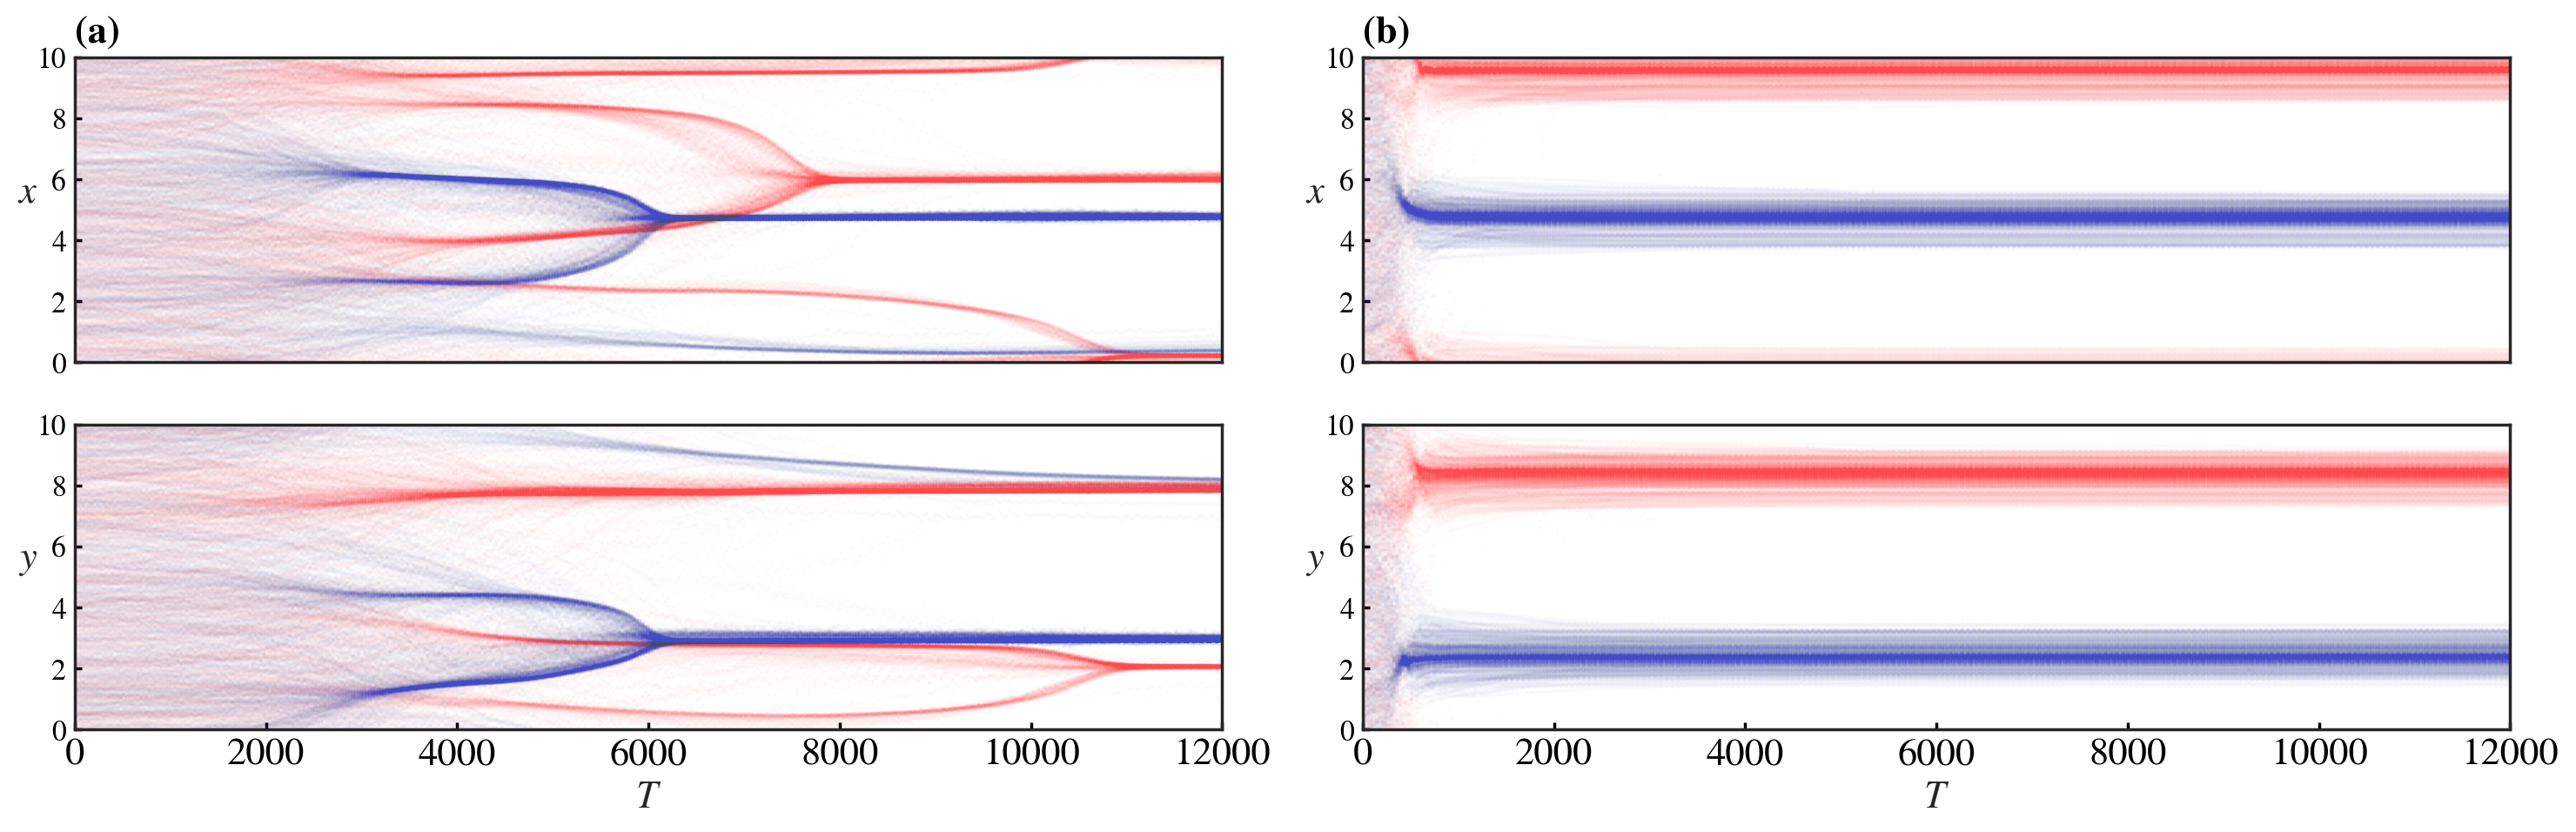
\includegraphics[width=\textwidth]{./figs/centersPosition.png}
    \caption{
        \label{fig:centersPosition} Scatter plot of the real-time centers position. 
        \textbf{(a)}, centers position of Ring ($\lambda=0.02$, $d_0=0.4$). As time goes on, the centers of oscillators with the same chirality converge.
        \textbf{(b)}, centers position of Swarm ($\lambda=0.01$, $d_0=2$). Unlike Ring, the centers converge quickly.
        The centers position are estimated with method in Fig.~\ref{fig:CenterEps} and Eq.~(\ref{eq:linearEquations}).
    }
\end{figure*}

\subsection{Disorder State}

Disorder state occurs when both $\lambda$ and $d_0$ are small. In this state, the oscillators are not asynchronous (phase histogram is uniform, like Fig.~\ref{fig:phaseHist}a) and move in a way which similar to uncoupled oscillators ($\lambda=0$), as shown in Fig.~\ref{fig:disorderState}a. According to Eq.~(\ref{eq:dotxi})-(\ref{eq:dotthetai}), when $\lambda=0$, the equations of oscillators' motion can be written as:
\begin{eqnarray}
    x_i\left( t \right) =x_{i}^{0}+\frac{v}{\omega _i}\sin \left[ \theta _i\left( 0 \right) +\omega _it \right] \;,\label{eq:circlemotionx}\\
    y_i\left( t \right) =y_{i}^{0}-\frac{v}{\omega _i}\cos \left[ \theta _i\left( 0 \right) +\omega _it \right] \;.
\end{eqnarray}

Then we have
\begin{equation}
    \left( x_i -x_{i}^{0} \right) ^2+\left( y_i -y_{i}^{0} \right) ^2=\left( \frac{v}{\omega _i} \right) ^2\;.
\end{equation}
In such a setup, oscillators move in a circular trajectory with radius $v/\omega _i$ and the phases $\theta_i$ increase linearly with time, as show in Fig.~\ref{fig:disorderState}b. To calculate the real-time rotational radius, we first estimate real-time centers $\mathbf{c}(t)$ of the circular trajectory with method in Fig.~\ref{fig:CenterEps} and then solve the following linear equations:

\begin{figure}[b]
    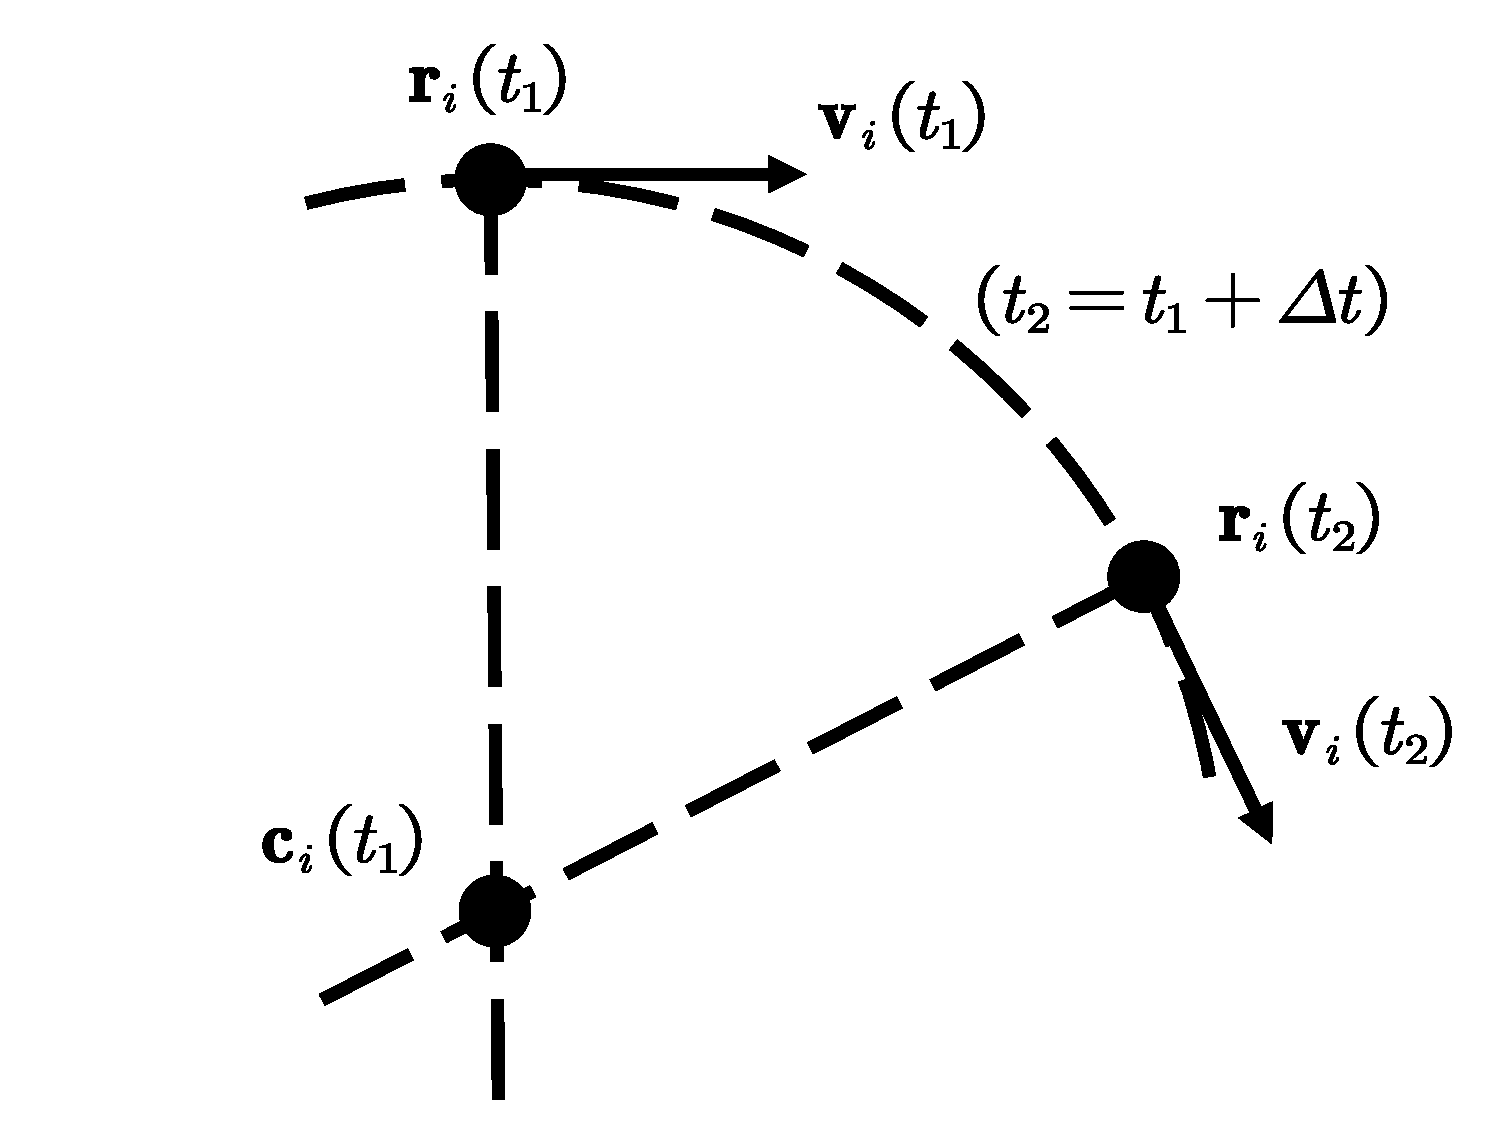
\includegraphics[width=0.25\textwidth]{./figs/CenterEps.pdf}
    \caption{\label{fig:CenterEps} Estimation for real-time centers.
    $\mathbf{c}_i(t_j)$, $\mathbf{r}_i(t_j)$ and $\mathbf{v}_i(t_j)$ are the center of the circular trajectory, the position and the velocity of the $i$th oscillator at time $t_j$, respectively.
    The line from $\mathbf{c}_i(t_j)$ to $\mathbf{r}_i(t_j)$ is perpendicular to $\mathbf{v}_i(t_j)$.}
\end{figure}

\begin{equation}\label{eq:linearEquations}
    \begin{array}{c}
        \mathbf{c}_i\left( t_1 \right) \cdot \mathbf{v}_i\left( t_1 \right) =\mathbf{x}_i\left( t_1 \right) \cdot \mathbf{v}_i\left( t_1 \right)\;,\\
        \mathbf{c}_i\left( t_2 \right) \cdot \mathbf{v}_i\left( t_2 \right) =\mathbf{x}_i\left( t_2 \right) \cdot \mathbf{v}_i\left( t_2 \right)\;,\\
    \end{array}
\end{equation}
where $\mathbf{v}_i(t_1)=\left( x_i\left( t_1 \right) , y_i\left( t_1 \right) \right)$ is the velocity of $i$th oscillator at $t_1$, and $\mathbf{v}_i(t_1)=\left( \cos \theta _i\left( t_1 \right) , \sin \theta _i\left( t_1 \right) \right)$ is the unit vector of the velocity. According to Eq.~(\ref{eq:dotxi})-(\ref{eq:dotthetai}), we can calculate $\mathbf{v}_i(t_2)$ and $\mathbf{r}_i(t_2)$, ($t_2=t_1+\Delta t$). 

The real-time rotational radius is $r_i(t)=\left| \mathbf{c}_i(t)-\mathbf{r}_i(t) \right|$. We found that the real-time rotational radius is almost constant and close to $v/\omega_i$ for each oscillator in the Disorder state, as shown in Fig.~\ref{fig:radiusOmega}a. The estimation results of four states' real-time rotational centers are shown in Fig.~\ref{fig:etimateCenter} in Appendix.

\subsection{Ring State}

The Ring state is characterized by the oscillators forming several rings with thickness, each of which is composed of oscillators with the same chirality, as is show in Fig.~\ref{fig:phaseDiagram}a. 
Similar to Disorder state, the oscillators in the same ring cluster move in a circular trajectory with a constant rotational radius calculated in Fig.~\ref{fig:radiusOmega}a. 
The oscillators' phase is uniformly distributed in the range $\left[ -\pi,\pi \right]$ (cf. Fig.~\ref{fig:phaseHist}a), which leads to oscillators uniformly located on the circular trajectory.
Fig.~\ref{fig:centersPosition}a shows there is a long transient time before this state is reached, and in this transient time, the trajectories of oscillators with the same chirality aggregate slowly. Conversely, the oscillators with different chirality repel each other. 

\begin{figure*}
    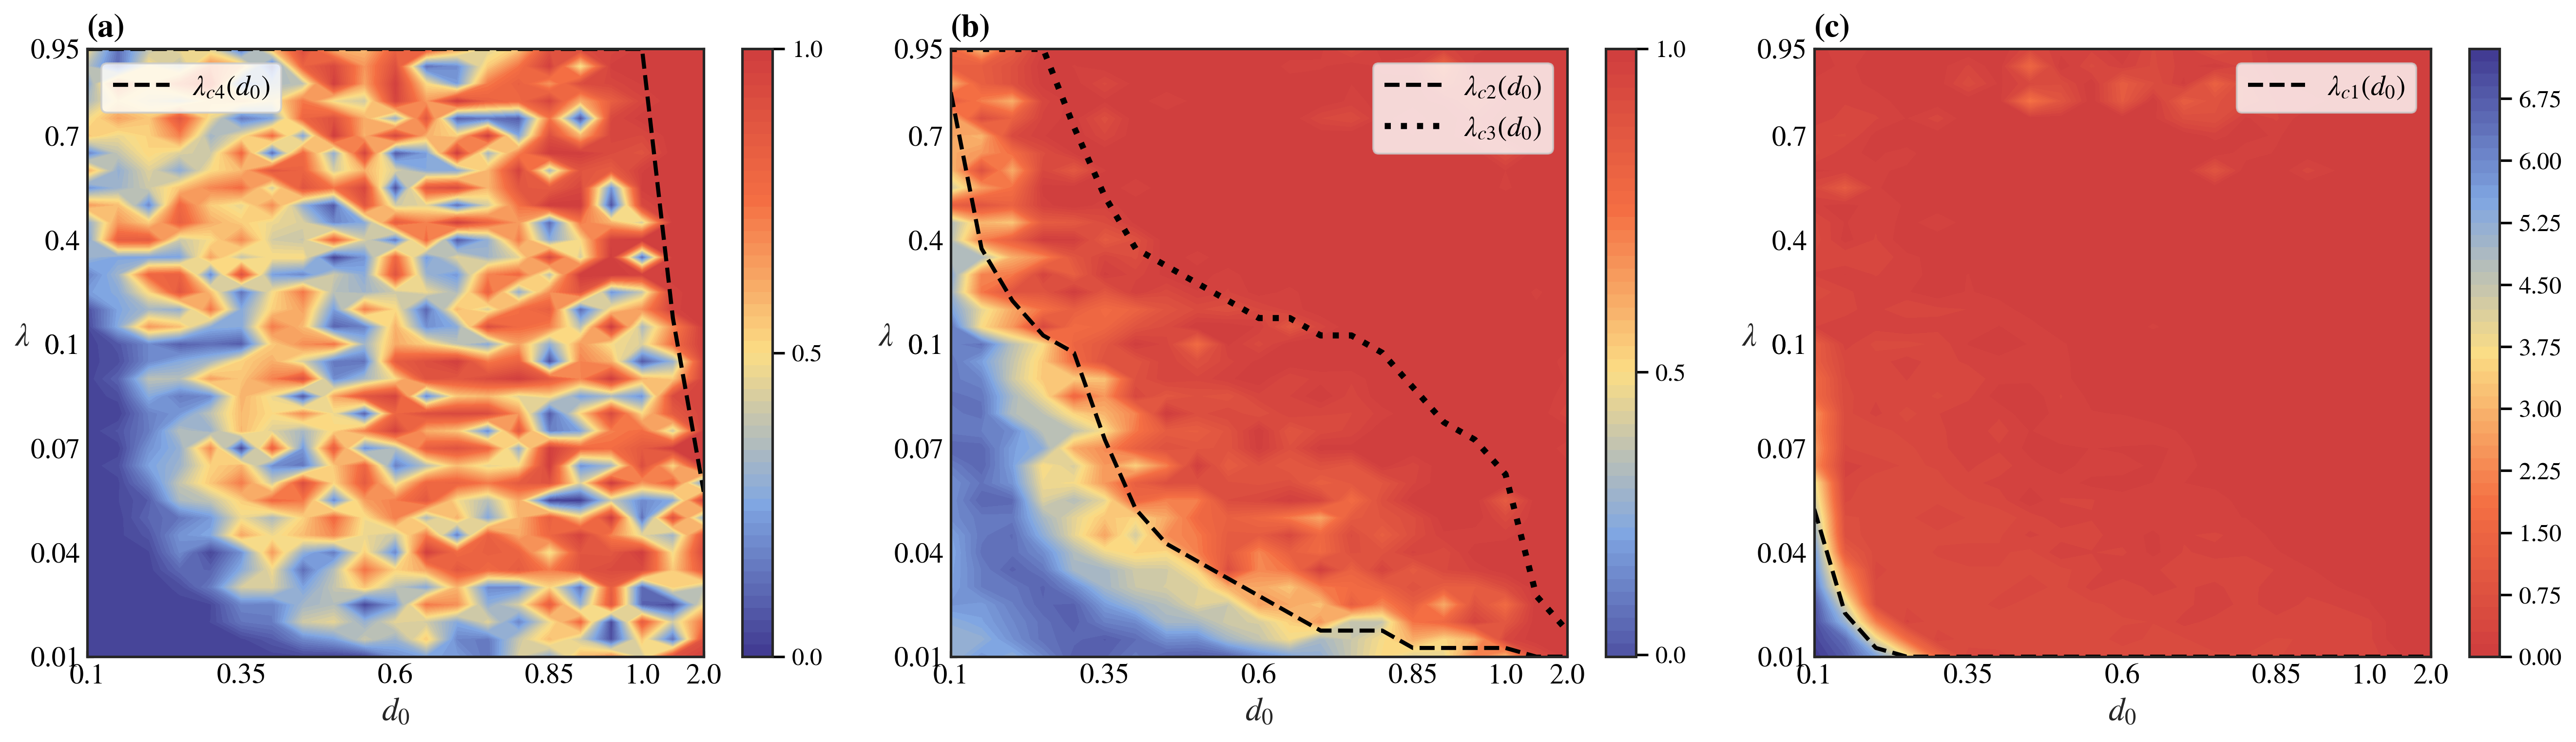
\includegraphics[width=\textwidth]{./figs/orderParam.png}
    \caption{
        \label{fig:orderParam} Order parameter heatmaps of ($\lambda$, $d_0$) plane and the critical lines of the transitions between states.
        \textbf{(a)}, order parameter $R$ and critical line of $\lambda_{c4}$.
        \textbf{(b)}, order parameter $R_s$ and critical lines of $\lambda_{c2}$, $\lambda_{c3}$.
        \textbf{(c)}, order parameter $\Delta \Omega$ and critical lines of $\lambda_{c1}$.
        All order parameters are calculated at $t=60000$.
    }
\end{figure*}

\subsection{Swarm State}

Swarm State is a state where the oscillators form spatial clusters and align into several clusters [Fig.~\ref{fig:phaseDiagram}b, c and Fig.~\ref{fig:centersPosition}b]. When $\lambda$ and $d_0$ increases, the number of clusters decreases by 2, which is named by Double-Clusters state, and other states are named by Multi-Clusters state. The clusters are composed of oscillators with the same chirality, and the phase $\theta_i$ of the oscillators in the same cluster is synchronized as seen in Fig.~\ref{fig:phaseHist}b and \ref{fig:phaseHist}c, which means that the oscillators in the cluster move with the same velocity $\mathbf{v}_i=\left( \cos \theta _s,\ \sin \theta _s \right)$ and rotational radius $r_i=v/\theta_s$, where $\theta_s$ is the oscillators' phase in the cluster. Based on this property, we can calculate $\theta_s$ and $r_i$ with Eq.~(\ref{eq:dotthetai}):

\begin{equation}\label{eq:clusterState}
    \begin{aligned}
        N_s\omega _s&=\sum_{i=1}^{N_s}{\left( \omega _i+\lambda \sum_{j=1}^{N_s}{A_{ij}\sin \left( \theta _j-\theta _i \right)} \right)}\\
        \omega _s&=\frac{1}{N_s}\sum_{i=1}^{N_s}{\omega _i}+\frac{\lambda}{N_s}\sum_{i=1}^{N_s}{\sum_{j=1}^{N_s}{A_{ij}\sin \left( \theta _j-\theta _i \right)}}\\
        &=\frac{1}{N_s}\sum_{i=1}^{N_s}{\omega _i}\;,\\
    \end{aligned}
\end{equation}
where $N_s$ is the number of oscillators in the cluster.
As $\omega_i \sim U\left( \omega _{\min},\omega _{\max} \right)$ and $\omega_i \sim U\left( -\omega _{\max},-\omega _{\min} \right)$ for two types of chirality, we can calculate $\theta_i$, $\omega_s$ and $r_i$ with $\omega_i$ for Double-Clusters state:

\begin{equation}
    \begin{aligned}\label{eq:clusterState2}
        \theta _i&=\omega _s=\begin{cases}
        \left( \omega _{\max}+\omega _{\min} \right) /2,&		i=1,2,\dots ,N/2\\
        -\left( \omega _{\max}+\omega _{\min} \right) /2,&		i=N/2+1,\cdots ,N\\
    \end{cases}\,\,,\\
        r_i&=\frac{v}{\left|\omega _s\right|}\;,\\
    \end{aligned}
\end{equation}
as shown in Fig.~\ref{fig:radiusOmega}b. But for Multi-Clusters, due to which oscillators are synchronized within each cluster is not accurately known, we can only calculate the real-time rotational radius of them. As seen in Fig.~\ref{fig:radiusOmega}b, similar to Double-Clusters, some local platforms appear in the real-time rotational radius due to synchronization.

\subsection{Quick Sync State}

Quick Sync state is a simple state where total oscillators are synchronized quickly, as shown in Fig.~\ref{fig:phaseDiagram}d. and \ref{fig:phaseHist}d. The oscillators are synchronized in an extremely short time, which leads them have no time to form clusters (can also be considered as a special case of Swarm state). Due to the two types of chirality oscillators are synchronized and the distributions of them is symmetric, the phase velocities of total oscillators are close to zero according to Eq.~(\ref{eq:clusterState}).

\section{\label{sec:orderParam}Order Parameter}

Having described the four states of our system, we next discuss how to distinguish them. We use the order parameter $R$ to measure global synchronization. The order parameter $R$ is defined as:

\begin{equation}
    R=\left| \frac{1}{N}\sum_{j=1}^N{e^{i\theta _j}} \right|\;.
\end{equation}
The order parameter $R$ is the absolute value of the mean of the complex numbers $e^{i\theta _i}$, which can be interpreted as the mean direction of the oscillators. When $R=1$, the oscillators are completely synchronized, and when $R=0$, the oscillators are completely desynchronized. Fig \ref{fig:orderParam}a shows the order parameter $R$ in the parameter plane. The order parameter $R$ is close to $1$ in the Quick Sync state, close to $0$ in the Disorder state and most of the Ring state, and between $0$ and $1$ in other states. In these states, we see that the order parameter $R$ changes non-monotonically in the sense that phases in these states are not globally synchronized, and each cluster's phase velocity $\omega_s\ne 0$. When the phases of different clusters are exactly equal, the order parameter $R$ is close to $1$, and when they are exactly opposite, $R$ is close to $0$.

Having realized that the order parameter $R$ is not enough to distinguish the states with clusters, we next define the following order parameter $R_s$ to metric the local synchronization,

\begin{figure}[b]
    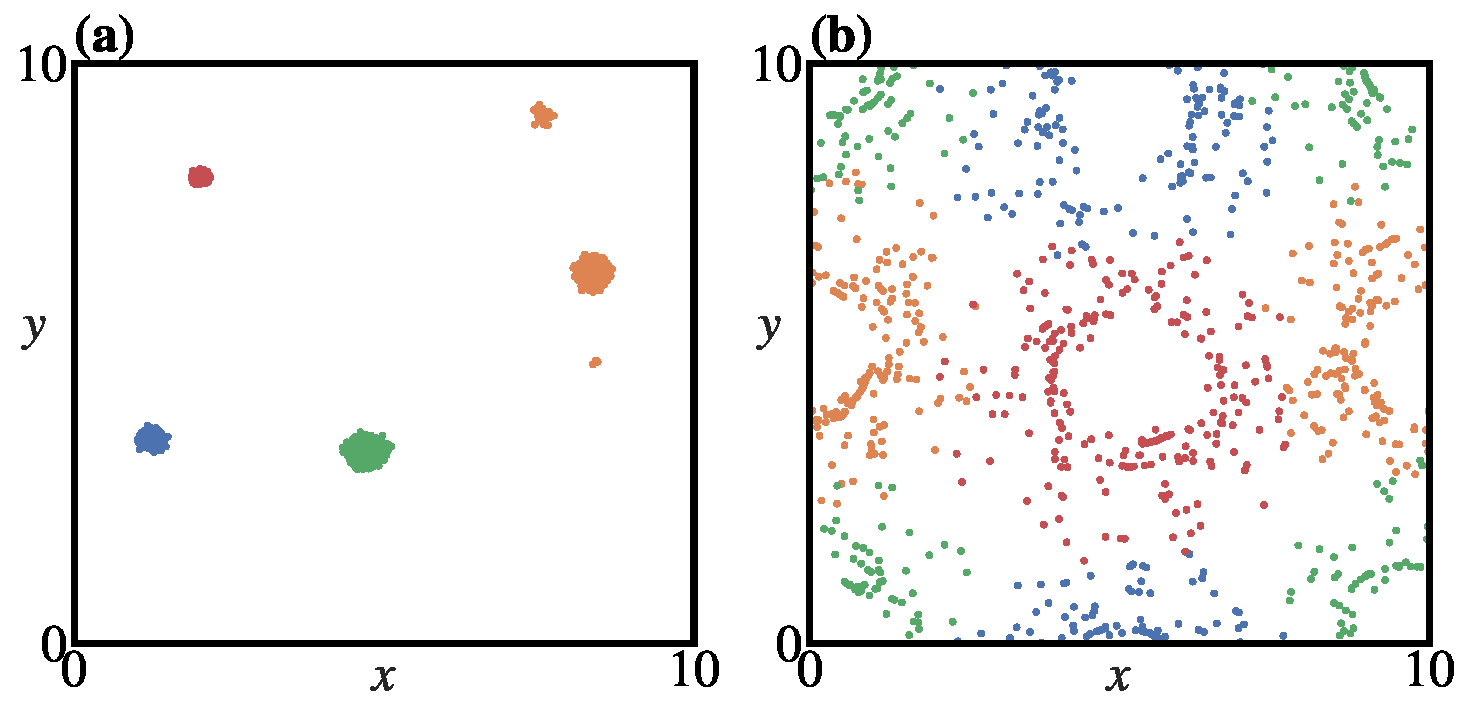
\includegraphics[width=0.48\textwidth]{./figs/classifyResult.pdf}
    \caption{
        \label{fig:classifyResult} Two examples of classification results. \textbf{(a)}: ($\lambda=0.4$, $d_0=0.3$). \textbf{(b)}: ($\lambda=0.02$, $d_0=0.4$).
    }
\end{figure}

\begin{equation}
    R_s=\frac{1}{N_c}\sum_{k=1}^{N_c}{\left| \frac{1}{\left| C_k \right|}\sum_{j\in C_k}{e^{i\theta _j}} \right|}\;,
\end{equation}
where $N_c$ is the number of clusters, $C_k$ is the $k$th cluster, and $\left| C_k \right|$ is the number of oscillators in the $k$th cluster. We can consider $R_s$ as an order parameter that studies the spatial position and internal phase simultaneously.
To determine the classification of clusters, we use the following method: we first calculate the relative center distance matrix $D_{ij}=\left| \mathbf{c}_i-\bar{\mathbf{c}}_j \right|$, where $\bar{\mathbf{c}}_j=\left( \bar{x}_j,\bar{y}_j \right)$ is the adjusted position of the $j$th oscillator's rotational center calculated by Eq.~(\ref{eq:adj_pos1}), (\ref{eq:adj_pos2}) and (\ref{eq:linearEquations}). 
The reason of using the distance between centers instead of the distance between oscillators' positions is that the oscillators in the Ring state are uniformly distributed on the circular trajectory, and the distance between them is much larger than the distance between their centers.
Then we use the DBSCAN algorithm to cluster the oscillators. The DBSCAN algorithm is a density-based clustering algorithm, which can find clusters of arbitrary shapes and sizes. We set the minimum number of oscillators in a cluster to be $5$ and the maximum distance between two oscillators in the same cluster to be $0.3$ (see Appendix \ref{sec:DBSCAN_param} for details on the determination of these parameters). 
One example of the classification of clusters is shown in Fig.~\ref{fig:classifyResult}.
We then calculate the order parameter $R_s$ for each cluster. The order parameter $R_s$ is close to $1$ in the Swarm state ($R_s$ of Double-Clusters state is closer to $1$ than Multi-Clusters) and Quick Sync state, and close to $0$ in Disorder state and most of the Ring state, between $0$ and $1$ in other Ring states with local clusters, as shown in Fig.~\ref{fig:orderParam}b.

Combining the order parameter $R$ and $R_s$, we can find only the distinction between Ring and Disorder states has not been resolved. Except the study for synchronization, we also define an order parameter $\Delta \Omega$ to metric the phase locking of the oscillators:

\begin{equation}
    \Delta \Omega =\frac{1}{N_c}\sum_{k=1}^{N_c}{\left[ \frac{1}{\left| C_k \right|^2}\sum_{i,j\in C_k}{\left( \left< \dot{\theta}_i \right> -\left< \dot{\theta}_j \right> \right) ^2} \right]}\;,
\end{equation}
where $\left< \dot{\theta}_i \right>$ is the average of the phase velocity of the $i$th cluster, which can be calculated by
\begin{equation}
    \left< \dot{\theta}_i \right> =\lim_{T\rightarrow \infty} \frac{1}{T}\int_{t_0}^{t_0+T}{\dot{\theta}_i\left( t \right) \mathrm{d}t}\;.
\end{equation}
We estimate $\left< \dot{\theta}_i \right>$ by the average of the phase velocity of the oscillators in the $i$th cluster at the last $1000$ time steps. 
The order parameter $\Delta \Omega > 0$ in the Disorder state, and $\Delta \Omega = 0$ in other states, as shown in Fig.~\ref{fig:orderParam}c.

To sum up, using $R$, $R_s$ and $\Delta \Omega$ in combination allows us to discern all the equilibrium state of our system.
The order parameter values in each state are summarized in Table \ref{tab:orderParam}.

\begin{table}
    \caption{\label{tab:orderParam} Order parameter values in each state 
    }
    \begin{ruledtabular}
        \begin{tabular}{lccc}
        State& $R$ & $R_s$ & $\Delta\Omega$ \\
        \hline
        Disorder&$=0$&$=0$&$> 0$\\
        Ring&$=0$&$=0$&$=0$\\
        Swarm (Multi-Clusters)&$> 0$&$\rightarrow 1$\footnotemark[1]&$=0$\\
        Swarm (Double-Clusters)&$> 0$&$\rightrightarrows 1\footnotemark[1]$&$=0$\\
        Quick Sync&$=1$&$=1$&$=0$\\
        \end{tabular}
    \end{ruledtabular}
    \footnotetext[1]{Note that the $R_s$ of Double-Clusters state is closer to $1$ than that of Multi-Clusters state.}
\end{table}

\begin{figure*}
    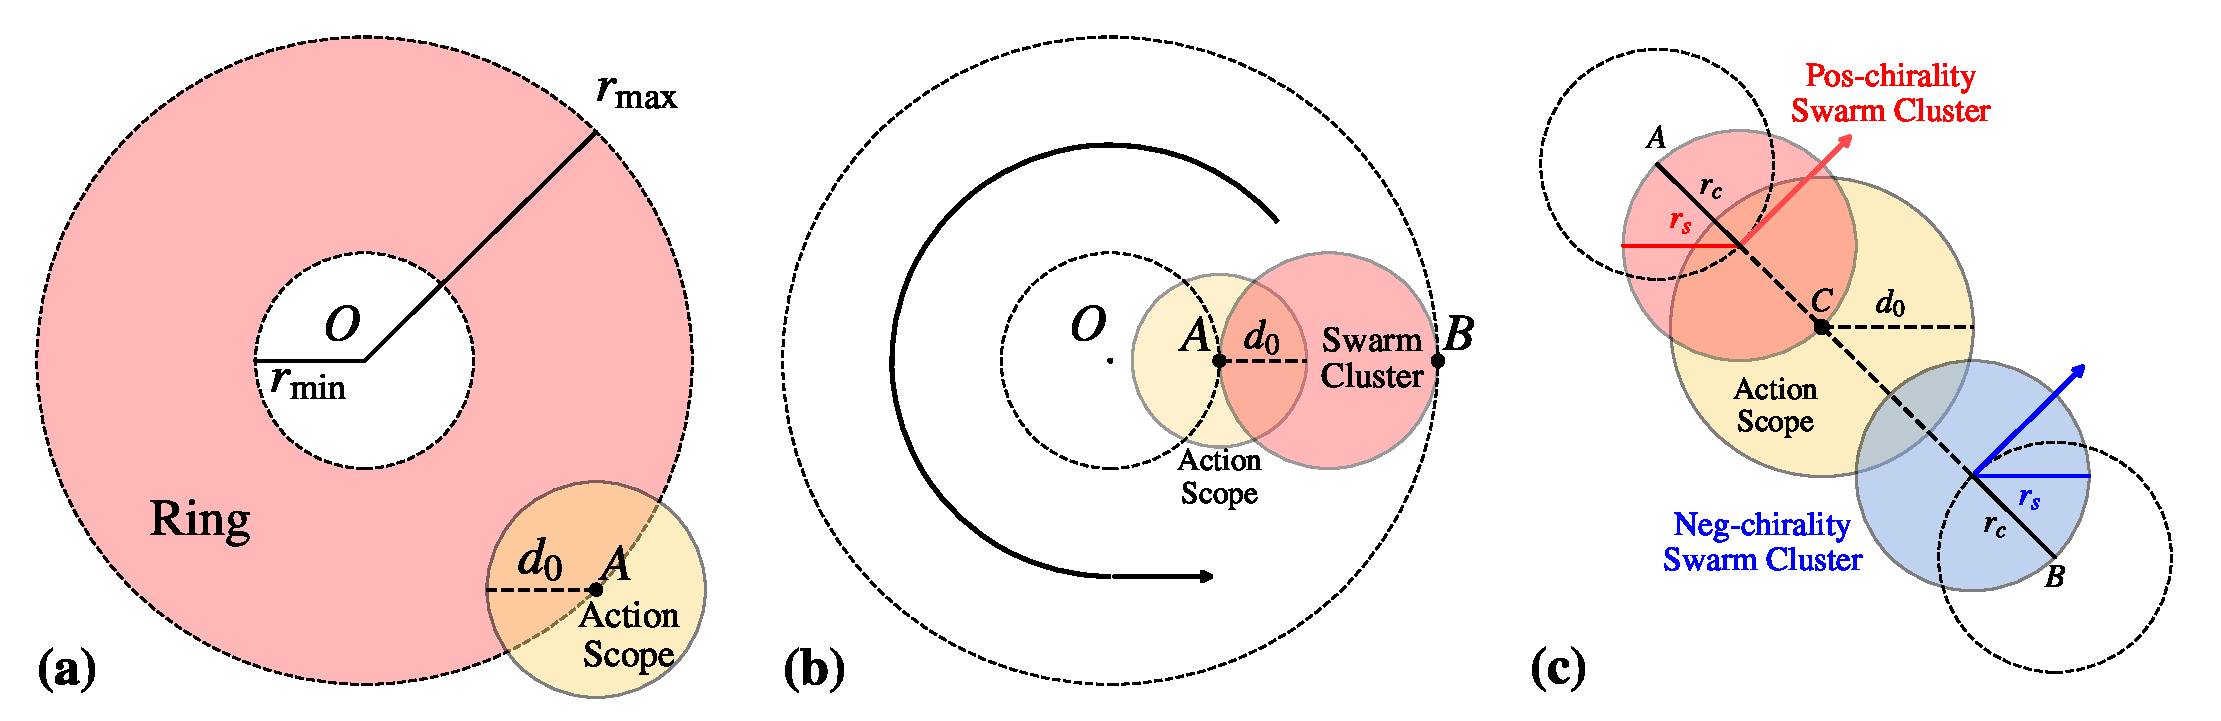
\includegraphics[width=\textwidth]{./figs/analyticalEps.pdf}
    \caption{
        \label{fig:analyticalEps}
        The schematic plot of the analytical approximations.
        \textbf{(a)}, The $1$st oscillator is at point $A$ which is on the outer edge of the ring, and the overlapping area of the yellow circle (action scope) and the red ring is $S_1\left( d_0 \right)$.
        \textbf{(b)}, The $1$st oscillator is at point $A$ which is on the inner edge of the ring, and the overlapping area of the yellow circle (action scope) and the red ring is $S_2\left( d_0 \right)$.
        \textbf{(c)}, The $1$st oscillator is at point $C$ which is on the edge of red circle, and the overlapping area of the yellow circle (action scope) and the blue circle is $S_3\left( d_0 \right)$.
    }
\end{figure*}

\section{\label{sec:analysis}Analytical approximations}

\subsection{\label{critical} Derivation of the critical boundaries}

In this section we derive the analytical approximations of the boundaries between the states. 
The boundaries between the states are determined by the critical lines $\lambda_{c1}$, $\lambda_{c2}$, $\lambda_{c3}$, and $\lambda_{c4}$, which are the critical values of $\lambda$ for the transitions between the states with given $d_0$.

\vspace{0.25cm}
\noindent\textbf{$\lambda_{c1}$: Disorder to Ring.}
We first consider the transition between the Disorder and Ring states. The oscillators in both states move in a circular trajectory (cf. Fig.~\ref{fig:disorderState}b), and the difference between them is that the oscillators in the Ring state are phase-locked.
Therefore, oscillators in Disorder state have a very small probability of being randomly distributed on the ring, but without phase locking.
The critical coupling strength $\lambda_{c1}$ can be calculated as the critical value of $\lambda$ for the phase locking of oscillators on the same ring.
We consider the following synchronous dynamics of oscillators on the same ring:
\begin{eqnarray}
    \dot{\theta}_1&=&\omega _1+\lambda \sum_{j=2}^{N_c}{A_{1j}\sin \left( \theta _j-\theta _1 \right)}\;,\label{eq:dotTheta1}
    \\
    \dot{\theta}_j&=&\omega _j\;,\label{eq:dotThetaj}
\end{eqnarray}
for $j=2,3,\ldots,N_c$, where $N_c$ is the number of oscillators on the same ring, and $\theta _1$ is the phase of the oscillator about to be phase-locked. Introducing the phase difference $\Delta \theta _j=\theta _j-\theta _1$ and $\Delta \omega _j=\omega _j-\omega _1$, we have:
\begin{equation}
    \label{eq:dotDeltaTheta}
    \Delta\dot{\theta}_j=\Delta \omega _j+\lambda \sum_{k=2}^{N_c}{A_{jk}\sin \Delta \theta _k}\;.
\end{equation}
Each oscillator only needs to be phase-locked with neighboring oscillators (minimum $\left| \Delta \omega _j \right|$) to achieve phase locking of entire ring due to the symmetry.
The minimum $\left| \Delta \omega _j \right|$ in a ring is $\left| \Delta \omega _j \right|=\left( \omega _{\max}-\omega _{\min} \right) /N_c$. When $\lambda \sum_{k=2}^{N_c}{A_{jk}} \geqslant \left| \Delta \omega _j \right|$, Eq.~(\ref{eq:dotDeltaTheta}) has fixed point solutions, and the oscillators are phase-locked. Therefore, the critical coupling strength $\lambda_{c1}$ is:
\begin{equation}
    \lambda _{c1}=\frac{\omega _{\max}-\omega _{\min}}{N_c\sum\nolimits_{j=2}^{N_c}{A_{1j}}}\;,
\end{equation}
where $\sum\nolimits_{j=2}^{N_c}{A_{1j}}$ is the number of oscillators within the action scope of the $1$st oscillator on the ring. Obviously, this is a function of $d_0$. We define it as
\begin{equation}
    N_1\left( d_0 \right) =N_c\frac{S_1\left( d_0 \right)}{S_R}=\frac{N_cS_1\left( d_0 \right)}{\pi \left( r_{\max}^{2}-r_{\min}^{2} \right)}\;,
\end{equation}
where $S_1$ is the overlapping area of the action scope of the $1$st oscillator and the ring, $S_R$ is the area of the ring, $N_c$ is the number of oscillators in the ring and $r_{\max}=v/\omega_{\min}$, $r_{\min}=v/\omega_{\max}$ are the outer, inner radius of the ring, respectively. In order to achieve phase locking of all oscillators on the ring, we need to consider the minimum value of $N_1\left( d_0\right)$. As shown in Fig.~\ref{fig:analyticalEps}a, the $1$st oscillator is at point $A$ which is on the outer edge of the ring, and the overlapping area of the yellow circle (action scope) and the red ring is $S_1\left( d_0 \right)$.  Elementary geometry gives 
\begin{equation}\label{eq:S1}
    \begin{cases}
        S_1\left( d_0 \right) =d_{0}^{2}\frac{\alpha}{2}+r_{\max}^{2}\frac{\beta}{2}-r_{\max}d_0\sin \frac{\alpha}{2}\\
        \beta =2\mathrm{arc}\cos \left( 1-\frac{d_{0}^{2}}{2r_{\max}^{2}} \right)\\
        \alpha =\pi -\frac{\beta}{2}\\
    \end{cases}\;,
\end{equation}
where $\alpha$ and $\beta$ are the angles of sectors from two overlapping circles' centers. Overall, we have
\begin{equation}
    \begin{cases}
        \lambda _{c1}=\frac{\pi \left( r_{\max}^{2}-r_{\min}^{2} \right) \left( \omega _{\max}-\omega _{\min} \right)}{N_{c}^{2}\left( d_{0}^{2}\frac{\alpha}{2}+r_{\max}^{2}\frac{\beta}{2}-r_{\max}d_0\sin \frac{\alpha}{2} \right)}\\
        \beta =2\mathrm{arc}\cos \left( 1-\frac{d_{0}^{2}}{2r_{\max}^{2}} \right)\\
        \alpha =\pi -\frac{\beta}{2}\\
    \end{cases}\;.
\end{equation}
Then we can calculate the critical line $\lambda_{c1}$ in the $(\lambda$-$d_0)$ plane with $N_c=250$ ($1/4$ of the total population $N=1000$), as shown in Fig.~\ref{fig:orderParam}c, where the line accurately divides the phase-locked and non-phase-locked regions, which is the critical line of the transition between the Disorder and Ring states. Here we set the number of oscillators in a ring $N_c=N/4$ because the maximum number of rings that an $L\times L$ box can accommodate is approximately
\begin{equation}
    \frac{L^2}{\pi r_{\max}^{2}}=3.54\;,
\end{equation}
which is $4$ after rounding.

\vspace{0.25cm}
\noindent\textbf{$\lambda_{c2}$: Ring to Swarm (Multi-Clusters).} According to $R_s$ in Fig.~\ref{fig:orderParam}b, the oscillators in the cluster are synchronized, and the oscillators with different chirality are not synchronized. Therefore, $\lambda_{c2}$ is the critical value of $\lambda$ for the synchronization of oscillators in the same cluster. We still consider the synchronous dynamics in Eq.~(\ref{eq:dotTheta1}) and (\ref{eq:dotThetaj}). To achieve synchronization, the oscillators with the largest phase difference (maximum $\left| \Delta \omega _j \right|$) in the cluster need to be phase-locked. The maximum $\left| \Delta \omega _j \right|$ in a cluster is $\left| \Delta \omega _j \right|=\omega _{\max}-\omega _{\min}$. Thus, the critical coupling strength $\lambda_{c2}$ is:
\begin{equation}
    \lambda _{c2}=\frac{\omega _{\max}-\omega _{\min}}{\sum\nolimits_{j=2}^{N_s}{A_{1j}}}\;,
\end{equation}
where $N_s$ is the number of oscillators in the cluster, and $\sum\nolimits_{j=2}^{N_s}{A_{1j}}$ is the number of oscillators within the action scope of the $1$st oscillator in the cluster, which is $N_2\left( d_0 \right)$. We define it as

\begin{equation}
    N_2\left( d_0 \right) =N_s\frac{S_2\left( d_0 \right)}{S_S}=\frac{N_sS_2\left( d_0 \right)}{\pi r_{s}^{2}}\;,
\end{equation}
where $S_2$ is the overlapping area of the action scope of the $1$st oscillator and the cluster, $S_S$ is the area of the cluster. Considering that this is a phase transition between ring and cluster states, the oscillator moves with a rotational radius in the ring state until it gathers into clusters, so the radius of the cluster $r_s$ is $(r_{\max}-r_{\min})/2$, as shown in Fig.~\ref{fig:analyticalEps}b. Similar to Eq.~(\ref{eq:S1}), the minimum overlapping area $S_2$ (overlapping area of two circles in Fig.~\ref{fig:analyticalEps}b) can be calculated as
\begin{equation}
    \begin{cases}
        S_2\left( d_0 \right) =d_{0}^{2}\frac{\alpha}{2}+r_{s}^{2}\frac{\beta}{2}-r_sd_0\sin \frac{\alpha}{2}\\
        \beta =2\mathrm{arc}\cos \left( 1-\frac{d_{0}^{2}}{2r_{s}^{2}} \right)\\
        \alpha =\pi -\frac{\beta}{2}\\
    \end{cases}\;.
\end{equation}
Therefore, we have

\begin{equation}
    \begin{cases}
        \lambda _{c2}=\frac{\pi r_{s}^{2}\left( \omega _{\max}-\omega _{\min} \right)}{N_S\left( d_{0}^{2}\frac{\alpha}{2}+r_{s}^{2}\frac{\beta}{2}-r_sd_0\sin \frac{\alpha}{2} \right)}\\
        \beta =2\mathrm{arc}\cos \left( 1-\frac{d_{0}^{2}}{2r_{s}^{2}} \right)\\
        \alpha =\pi -\frac{\beta}{2}\\
        r_s=\frac{r_{\max}-r_{\min}}{2}\\
    \end{cases}\;.
\end{equation}
Then we can calculate the critical line $\lambda_{c2}$ in the $(\lambda$-$d_0)$ plane with $N_s=500$ (each chirality has half of the total population $N=1000$), as shown in Fig.~\ref{fig:orderParam}b, where the line divides whether local synchronization occurred.

\vspace{0.25cm}
\noindent\textbf{$\lambda_{c3}$: Multi-Clusters to Double-Clusters.} 
The derivation of $\lambda_{c3}$ is similar to that of $\lambda_{c2}$, but the difference is that the centers of oscillators in the Swarm (Double-Clusters) state converge quickly (cf Fig.~\ref{fig:centersPosition}b), which means oscillators do not require a long transient to form clusters. We consider that the oscillator density $\rho$ (Number of oscillators per unit area) under initial conditions can achieve synchronization of oscillators of the same chirality. $\rho$ can be calculated as 
\begin{equation}
    \rho =\frac{N}{L^2}\;.
\end{equation}
Then we have 
\begin{eqnarray}
    \sum_{j=2}^{N_c}{A_{1j}}=\rho \pi d_{0}^{2}=\frac{N\pi d_{0}^{2}}{L^2}\;.
\end{eqnarray}
The critical coupling strength $\lambda_{c3}$ is:
\begin{equation}
    \lambda _{c3}=\frac{L^2\left( \omega _{\max}-\omega _{\min} \right)}{N\pi d_{0}^{2}}\;.
\end{equation}
Similarly, we can calculate the critical line $\lambda_{c3}$ in the $(\lambda$-$d_0)$ plane, as shown in Fig.~\ref{fig:orderParam}b, where the values of region above the line (Double-Clusters) is closer to $1$ than below the line (Multi-Clusters).

\vspace{0.25cm}
\noindent\textbf{$\lambda_{c4}$: Swarm (Double-Clusters) to Quick Sync.}
The Quick Sync state can be considered as a special case of the Swarm state where the oscillators are globally synchronized. We assume that the oscillators of two chirality have been synchronized in the Swarm (Double-Clusters) state, as is shown in Fig.~\ref{fig:analyticalEps}c. Next, we consider the synchronization of the two chirality. According to Eq.~(\ref{eq:clusterState2}), two clusters with opposite chirality are moving on their respective circular trajectories with the same rotational radius
\begin{equation}
    r_c = \cfrac{2v}{\omega_{\max}+\omega_{\min}}\;.
\end{equation}
In numerical simulations, we observe that the radius $r_s$ of clusters in Swarm state increases with the increase of $\lambda$ and $d_0$. Thus, the radius of the clusters reach maximum value of $r_c$ (see proof in Appendix \ref{sec:maxRadius}) when the $\lambda$ and $d_0$ reach the critical values.

Considering that the trajectories of two chirality will repel each other before oscillators achieving global synchronization, let's take the maximum relative distance between the motion trajectories of two clusters in space, which is line $AB$ in Fig.~\ref{fig:analyticalEps}c. The distance $l_{AB}$ is
\begin{equation}
    l_{AB}=\frac{L}{\sqrt{2}}\;.
\end{equation}

Similar to the derivation of $\lambda_{c2}$, we consider the synchronization dynamics between a single oscillator ($C$ in Fig.~\ref{fig:analyticalEps}c) and a cluster (blue circle in Fig.~\ref{fig:analyticalEps}c), the difference is that the single oscillator and cluster here belong to different chirality. When the centers of two clusters move onto line segment AB, their distance is the shortest. At this point, due to symmetry, if the oscillators at the edges of the two clusters are synchronized, global synchronization can be achieved. Obviously, when 

\begin{equation}
    d_0+2r_c+2r_s<l_{AB}\;,
\end{equation}
the action scope of oscillator at point $C$ does not overlap with the neg-chirality cluster (blue circle), so the critical coupling strength $\lambda_{c4}$ does not exist. When $d_0+2r_c+2r_s>l_{AB}$, the overlapping area $S_3\left( d_0 \right)$ can be calculated as
\begin{equation}
    \begin{cases}
        S_3\left( d_0 \right) =r_{s}^{2}\frac{\alpha}{2}+d_{0}^{2}\frac{\beta}{2}-d_0r_d\sin \frac{\beta}{2}\\
        r_d=\frac{L}{\sqrt{2}}-r_s-2r_c\\
        \beta =2\mathrm{arc}\cos \frac{d_{0}^{2}+r_{d}^{2}-r_{s}^{2}}{2d_0r_d}\\
        \alpha =2\mathrm{arc}\cos \frac{r_{s}^{2}+r_{d}^{2}-d_{0}^{2}}{2r_sr_d}\\
    \end{cases}\;,
\end{equation}
where $r_s=r_c$. The global maximum value of $\left| \Delta \omega _j \right|$ is $\omega _{\max}-\left( -\omega _{\max} \right) =2\omega _{\max}$. Therefore, we have

\begin{equation}
    \begin{cases}
        \lambda _{c4}=\frac{2\pi r_{s}^{2}\omega _{\max}}{N_c\left( \frac{\alpha}{2}r_{s}^{2}+\frac{\beta}{2}d_{0}^{2}-d_0r_d\sin \frac{\beta}{2} \right)}\\
        r_d=\frac{L}{\sqrt{2}}-r_s-2r_c\\
        \beta =2\mathrm{arc}\cos \frac{d_{0}^{2}+r_{d}^{2}-r_{s}^{2}}{2d_0r_d}\\
        \alpha =2\mathrm{arc}\cos \frac{r_{s}^{2}+r_{d}^{2}-d_{0}^{2}}{2r_sr_d}\\
    \end{cases}\;.
\end{equation}
Then we can calculate the critical line $\lambda_{c4}$ in the $(\lambda$-$d_0)$ plane, as shown in Fig.~\ref{fig:orderParam}a, where the line divides whether global synchronization occurred. 

\subsection{Repulsion-attraction dynamics from phase coupling}

\begin{figure}[b]
    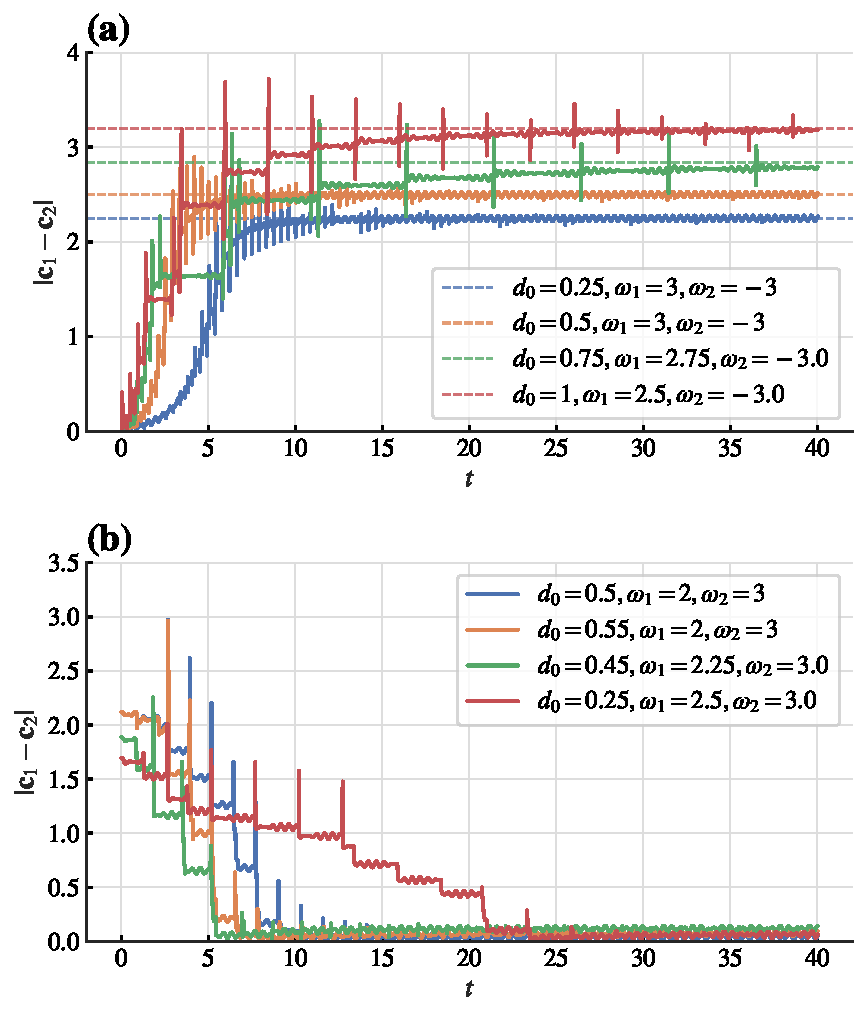
\includegraphics[width=0.48\textwidth]{./figs/2OsCenterDistance.pdf}
    \caption{
        \label{fig:2OsCenterDistance} The distance between the centers of two oscillators ($\lambda=1$). 
        \textbf{(a)}, The distance between the centers of two oscillators with the different chirality. The dashed line is the theoretical maximum distance of Eq~(\ref{eq:maxDistance}).
        \textbf{(b)}, The distance between the centers of two oscillators with the same chirality.
    }
\end{figure}

In the Ring state, the oscillators of two chirality exhibit a spatial repulsion-attraction mechanism driven by phase coupling. Specifically, the motion trajectories of oscillators with the same chirality are attracted to each other, while the motion trajectories of oscillators with different chirality repel each other (cf. Fig.~\ref{fig:centersPosition}a). 
In this subsection, We analyze the repulsion-attraction dynamics by considering the centers of oscillators' motion trajectories with a semi-analytic approximation.

According to the estimation method in Fig.~\ref{fig:CenterEps} and Eq.~(\ref{eq:linearEquations}), for the time of $t$ and $t+\mathrm{d}t, \mathrm{d}t\rightarrow 0$, the line connecting the rotational center $\mathbf{c}=(X,Y)$ and position $\mathbf{r}=(x,y)$ of the oscillator is perpendicular to the direction of velocity $\mathbf{v}$, then we have
\begin{eqnarray}
        &&\mathbf{v}\left( t \right) \cdot \left[ \mathbf{r}\left( t \right) -\mathbf{c} \right] =0\;,\label{eq:linearEquations1}
        \\
        &&\mathbf{v}\left( t+\mathrm{d}t \right) \cdot \left[ \mathbf{r}\left( t+\mathrm{d}t \right) -\mathbf{c} \right] =0\;.\label{eq:linearEquations2}
\end{eqnarray}
The Eq.~(\ref{eq:linearEquations2}) can be expanded as
\begin{equation}\label{eq:linearEquations2Exp}
    \begin{aligned}
        &\mathbf{v}\left( t \right) \cdot \mathbf{r}\left( t \right) +\left[ \mathbf{v}\left( t \right) \cdot \dot{\mathbf{r}}\left( t \right) +\dot{\mathbf{v}}\left( t \right) \cdot \mathbf{r}\left( t \right) \right] \mathrm{d}t+\dot{\mathbf{v}}\left( t \right) \cdot \dot{\mathbf{r}}\left( t \right) \mathrm{d}t^2 \\
        &=\mathbf{v}\left( t \right) \cdot \mathbf{c}+\dot{\mathbf{v}}\left( t \right) \mathrm{d}t\cdot \mathbf{c}\;.
    \end{aligned}
\end{equation}
Introduce Eq.~(\ref{eq:linearEquations1}) into Eq.~(\ref{eq:linearEquations2Exp}) and neglect the higher-order terms of $\mathrm{d}t$, we have
\begin{equation}
    \mathbf{v}\left( t \right) \cdot \dot{\mathbf{r}}\left( t \right) +\dot{\mathbf{v}}\left( t \right) \cdot \mathbf{r}\left( t \right) =\dot{\mathbf{v}}\left( t \right) \cdot \mathbf{c}
\end{equation}
Therefore, the linear equations can be written as
\begin{equation}
    \begin{aligned}
        &\mathbf{v}\left( t \right) \cdot \mathbf{r}\left( t \right) =\dot{x}\left( t \right) X\left( t \right) +\dot{y}\left( t \right) Y\left( t \right) \;,\\
        \frac{\mathrm{d}}{\mathrm{d}t}&\mathbf{v}\left( t \right) \cdot \mathbf{r}\left( t \right) =\ddot{x}\left( t \right) X\left( t \right) +\ddot{y}\left( t \right) Y\left( t \right)\;.\\
    \end{aligned}
\end{equation}
Solve the linear equations, we have
\begin{equation}\label{eq:linearSolve}
    \begin{aligned}
        X\left( t \right) &=x\left( t \right) -\frac{v}{\dot{\theta}\left( t \right)}\sin \theta \left( t \right)\;,\\
        Y\left( t \right) &=y\left( t \right) +\frac{v}{\dot{\theta}\left( t \right)}\cos \theta \left( t \right)\;.\\
    \end{aligned}
\end{equation}
Taking the derivative of Eq.~(\ref{eq:linearSolve}), we can get the velocity of the center
\begin{equation}
    \begin{aligned}
        \dot{X}\left( t \right) &=\frac{v\ddot{\theta}\left( t \right)}{\dot{\theta}^2\left( t \right)}\sin \theta \left( t \right)\;,\\
        \dot{Y}\left( t \right) &=-\frac{v\ddot{\theta}\left( t \right)}{\dot{\theta}^2\left( t \right)}\cos \theta \left( t \right)\;.\\
    \end{aligned}
\end{equation}

Due to the symmetry of the ring, we can consider the interaction between only two oscillators. 
According to the behaviors of the Ring state, the centers are ultimately static. Therefore, the distance between the centers of two oscillators will converge to a certain value. Only when $\ddot{\theta}_i$ and $\ddot{\theta}_j$ are zero
\begin{equation}\label{eq:staticCenter}
    \begin{aligned}
        \ddot{\theta}_i&=\lambda A_{ij}\left( \dot{\theta}_j-\dot{\theta}_i \right) \cos \left( \theta _j-\theta _i \right) =0\;,\\
        \ddot{\theta}_j&=\lambda A_{ij}\left( \dot{\theta}_i-\dot{\theta}_j \right) \cos \left( \theta _i-\theta _j \right) =0\;,\\
    \end{aligned}
\end{equation}
the centers will be static. $\dot{\theta}_i=\dot{\theta}_j$, $\theta _i-\theta _j=\pm\pi/2$ and $A_{ij}=0$ are the solutions of the Eq.~(\ref{eq:staticCenter}).

For the oscillators with the different chirality, the conditions of $\dot{\theta}_i=\dot{\theta}_j$ and $\theta _i-\theta _j=\pm\pi/2$ are not satisfied, due to $2\omega _{\min}>2\lambda $ (the coupling strength is not strong enough to lock the phase, even for the smallest natural frequency difference). Therefore, only when $A_{ij}=0$, which means the oscillators are not within the action scope of each other at any time, the centers of oscillators with different chirality will be static. 

For the oscillators with the same chirality, the conditions of $\dot{\theta}_i=\dot{\theta}_j$ and $\theta _i-\theta _j=\pm\pi/2$ can be satisfied when $\left| \Delta \omega \right|\leqslant 2\lambda$. The condition of $A_{ij}=0$ is only satisfied when two oscillators are not within the action scope of each other for beginning, otherwise the attraction of the same chirality will make the centers of oscillators converge to a minimum distance of $0$. In this case, $A_{ij}$ will not be zero at any time. 

Next, we analyze the reasons why the centers of oscillators with the same/ different chirality will converge to the two static states mentioned above.
For the $i$th and $j$th oscillators, the distance between their rotation centers is
\begin{equation}\label{eq:distanceCenter}
    \left| \mathbf{c}_j-\mathbf{c}_i \right|=\sqrt{\begin{array}{l}
        \left( x_j-\frac{v}{\dot{\theta}_j}\sin \theta _j-x_i+\frac{v}{\dot{\theta}_i}\sin \theta _i \right) ^2+\\
        \left( y_j+\frac{v}{\dot{\theta}_j}\cos \theta _j-y_i-\frac{v}{\dot{\theta}_i}\cos \theta _i \right) ^2\\
    \end{array}}\;.
\end{equation}
Then we can calculate the derivative of $\left| \mathbf{c}_j-\mathbf{c}_i \right|^2$

\begin{equation}\label{eq:distanceCenterDerivative}
    \frac{\mathrm{d}}{\mathrm{d}t}\left| \mathbf{c}_j-\mathbf{c}_i \right|^2=A+B+C\;,
\end{equation}
where 
\begin{eqnarray}
    &&\begin{aligned}
        A&=2\left[ \frac{v\ddot{\theta}_i}{\left( \dot{\theta}_i \right) ^2}\sin \theta _i-\frac{v\ddot{\theta}_j}{\left( \dot{\theta}_j \right) ^2}\sin \theta _j \right] \left( x_i-x_j \right)\\
        &\;+2\left[ -\frac{v\ddot{\theta}_i}{\left( \dot{\theta}_i \right) ^2}\cos \theta _i+\frac{v\ddot{\theta}_j}{\left( \dot{\theta}_j \right) ^2}\cos \theta _j \right] \left( y_i-y_j \right)\\
    \end{aligned}\\
	&&B=-2v^2\left[ \frac{\ddot{\theta}_i}{\left( \dot{\theta}_i \right) ^3}+\frac{\ddot{\theta}_j}{\left( \dot{\theta}_j \right) ^3} \right]\\
	&&C=\frac{2v^2}{\dot{\theta}_j\dot{\theta}_i}\left( \frac{\ddot{\theta}_i}{\dot{\theta}_i}+\frac{\ddot{\theta}_j}{\dot{\theta}_j} \right) \cos \left( \theta _i-\theta _j \right)
\end{eqnarray}

For $A$, since the coupling occurs only when the spatial distance is less than $d_0$, and the $d_0$ of the Ring state is small, the absolute value of $A$ is very small. To verify this, we calculate the value of $|B+C|-|A|$ in the Ring state. As shown in Fig.~\ref{fig:2OsBCsubA}, the value of $|B+C|-|A|>0$ for most of the time. Even if $|B+C|-|A|<0$, the absolute value is very small. Therefore, the Eq.~(\ref{eq:distanceCenterDerivative}) is mainly determined by $B$ and $C$.

\begin{figure}[b]
    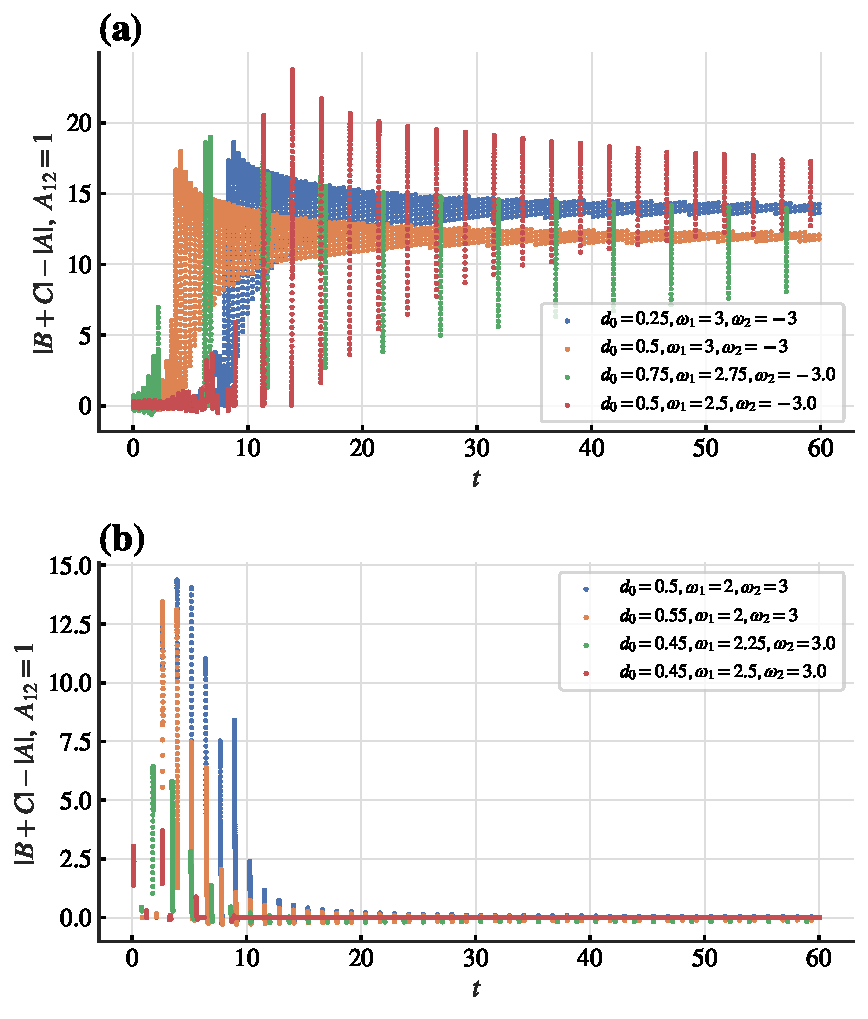
\includegraphics[width=0.48\textwidth]{./figs/2OsBCsubA.pdf}
    \caption{
        \label{fig:2OsBCsubA} The value of $|B+C|-|A|$ of two oscillators when $A_{ij}=1$ and $\lambda=1$.
        \textbf{(a)}, oscillators with the different chirality.
        \textbf{(b)}, oscillators with the same chirality.
    }
\end{figure}

For $B$, we can get $\ddot{\theta}_i=-\ddot{\theta}_j$ from Eq.~(\ref{eq:staticCenter}). Then $B$ can be written as
\begin{equation}
    B=-\frac{2v^2\lambda A_{ij}\left( \dot{\theta}_j-\dot{\theta}_i \right) ^2}{\left( \dot{\theta}_i\dot{\theta}_j \right) ^2}\left( 1+\frac{\dot{\theta}_j}{\dot{\theta}_i}+\frac{\dot{\theta}_i}{\dot{\theta}_j} \right) \cos \left( \theta _j-\theta _i \right)\;.
\end{equation}
Since $\lambda<|\omega_{\min}|$, we have $\text{sgn}\dot{\theta}_i=\text{sgn}\omega_i$, which means $\dot{\theta}_i$ and $\dot{\theta}_j$ have the same sign. So it is easy to see that
\begin{equation}
    \left( 1+\frac{\dot{\theta}_j}{\dot{\theta}_i}+\frac{\dot{\theta}_i}{\dot{\theta}_j} \right) \in \begin{cases}
        \left( 2,+\infty \right) ,&		\dot{\theta}_j\dot{\theta}_i>0\\
        \left( -\infty , 0 \right) ,&		\dot{\theta}_j\dot{\theta}_i<0\\
    \end{cases}\;.
\end{equation}
Therefore, we have
\begin{equation}
    \text{sgn} B =\begin{cases}
        -\text{sgn} \left( \cos \left( \theta _j-\theta _i \right) \right) ,&		\dot{\theta}_j\dot{\theta}_i\geqslant 0\\
        \text{sgn} \left( \cos \left( \theta _j-\theta _i \right) \right) ,&		\dot{\theta}_j\dot{\theta}_i<0\\
    \end{cases}\;.
\end{equation}
As time $t$ increases, the coupling causes the decrease of $\left| \theta _j-\theta _i \right|$. Therefore, as the absolute value of phase difference gradually decreases to within $\pi/2$, the sign of $B$ is negative for the oscillators with same chirality, and positive for different chirality.

For $C$, it can be written as
\begin{equation}
    C=2v^2\frac{\lambda A_{ij}\left( \dot{\theta}_j-\dot{\theta}_i \right) ^2\cos ^2\left( \theta _j-\theta _i \right)}{\left( \dot{\theta}_i\dot{\theta}_j \right) ^2}\;.
\end{equation}
This term is always positive. Since
\begin{equation}
    \left| \dot{\theta}_j-\dot{\theta}_i \right|=\begin{cases}
        \max \left\{ \dot{\theta}_i,\dot{\theta}_i \right\} -\min \left\{ \dot{\theta}_i,\dot{\theta}_i \right\} ,&		\dot{\theta}_j\dot{\theta}_i\geqslant 0\\
        \left| \dot{\theta}_j \right|+\left| \dot{\theta}_i \right|,&		\dot{\theta}_j\dot{\theta}_i<0\\
    \end{cases}\;,
\end{equation}
and $\left| \dot{\theta}_j \right|+\left| \dot{\theta}_i \right|\geqslant \max \left\{ \dot{\theta}_i,\dot{\theta}_i \right\} -\min \left\{ \dot{\theta}_i,\dot{\theta}_i \right\}$, the absolute value of $C$ for the oscillators with the different chirality is always larger than that for the same chirality.

In summary, when the coupling occurs, the distance between the rotation centers of two oscillators with the same signs of natural frequency $\omega$ (chirality) will decrease, which means the oscillators of the same chirality are attracted to each other, while the distance between the centers with opposite signs of $\omega$ (chirality) will increase, which means the oscillators of different chirality repel each other. 

\begin{figure}[b]
    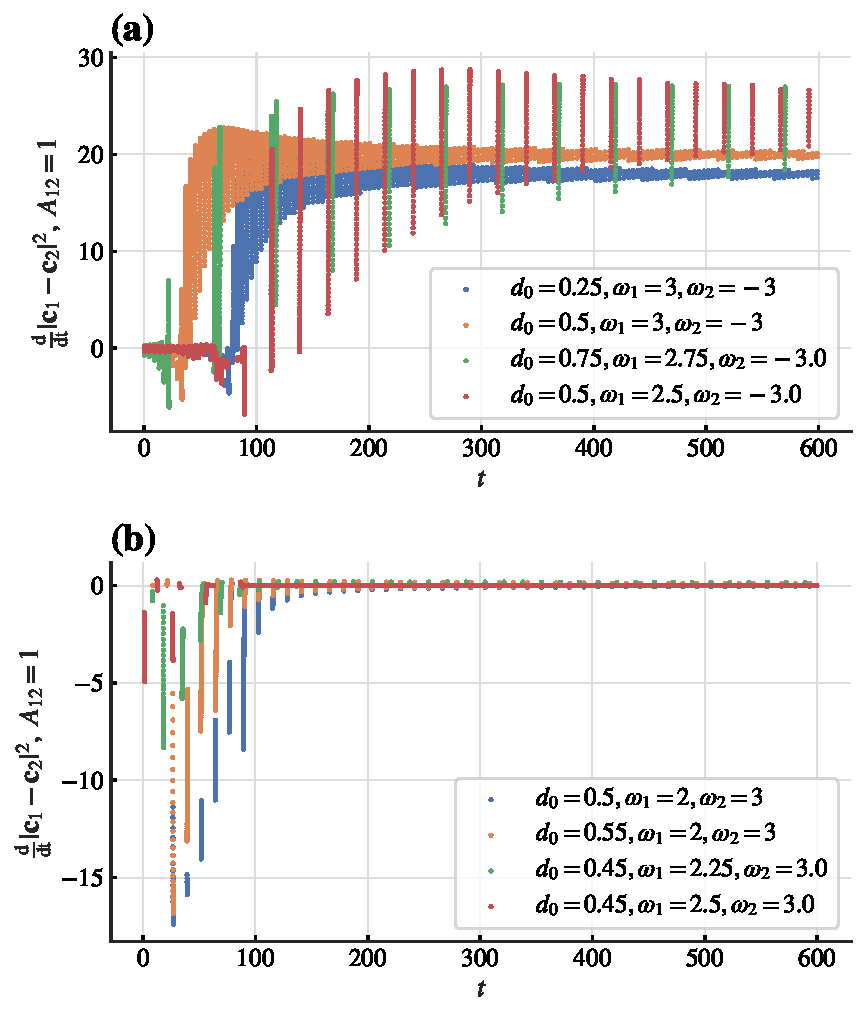
\includegraphics[width=0.48\textwidth]{./figs/2OsDotDistance.pdf}
    \caption{
        \label{fig:2OsDotDistance} The derivative of $\left| \mathbf{c}_j-\mathbf{c}_i \right|^2$ ($\lambda=1$).
        \textbf{(a)}, oscillators with the different chirality.
        \textbf{(b)}, oscillators with the same chirality.
    }
\end{figure}

Affected by this repulsive force, the distance between the centers of oscillators with different chirality will repel each other to a maximum distance. It is not difficult to imagine that the farthest distance is the distance where two oscillators happen to be unable to couple, so we assume that 
\begin{equation}
    \begin{array}{c}
        \lim_{t\rightarrow \infty ,A_{ij}=1} \left( \dot{\theta}_i-\dot{\theta}_j \right) =0\\
        \lim_{t\rightarrow \infty ,A_{ij}=1} \left( \theta _i-\theta _j \right) =0\\
    \end{array}\;.
\end{equation} 
Therefore, the long time solutions of $\left| \mathbf{c}_j-\mathbf{c}_i \right|^2$ is 
\begin{equation}
    \begin{aligned}
        \lim_{t\rightarrow \infty} \left| \mathbf{c}_j-\mathbf{c}_i \right|^2&=d_{ij}^{2}+\left( \frac{v}{\dot{\theta}_i}-\frac{v}{\dot{\theta}_j} \right) ^2\pm 2d_{ij}\left( \frac{v}{\dot{\theta}_i}-\frac{v}{\dot{\theta}_j} \right)\\
        &=\left[ \frac{v}{\dot{\theta}_i}-\frac{v}{\dot{\theta}_j}\pm d_{ij} \right] ^2\\
    \end{aligned}\;,
\end{equation}
For the oscillators with the different chirality, the maximum distance is 
\begin{equation}\label{eq:maxDistance}
    d_0+v/\left| \omega _1 \right|+v/\left| \omega _2 \right|\;.
\end{equation} 
Moreover, the distance between the centers of oscillators with the same chirality will be attracted to each other to a minimum distance of $0$. In this case, the radius of action cannot be too large to avoid two oscillators locking phase, otherwise the centers will not be able to reach $0$.
In Fig.~\ref{fig:2OsCenterDistance}, we show the distance between the centers of two oscillators with same or different chirality. They eventually converged to their theoretical maximum or minimum values.

\section{\label{sec:conclusions}CONCLUSIONS}

In summary, we have studied the collective dynamics of a system of coupled oscillators with diverse topologies. 
Most previous work on collective behavior directly defined the interaction forces between oscillators in space. Our research has introduced a simple model that couples the oscillators in phase space and the governing equations of space only indirectly affect the phase coupling. We found that even this simple model can exhibit rich collective dynamics.
We have identified five distinct states: Disorder, Ring, Swarm (which can be further divided into Multi-Clusters and Double-Clusters), and Quick Sync. 
The transitions between these states were shown driven by the coupling strength $\lambda$ and the action radius $d_0$. 
To distinguish these states, we have introduced three order parameters according to the collective behavior of the system: $R$ for the global synchronization of the system, $R_s$ for the synchronization of oscillators within the cluster and $\Delta\Omega$ for the phase-locking of oscillators on the same ring.
Furthermore, We have derived the analytical approximations of the critical boundaries between the states, which are found to be in good agreement with the numerical results and order parameters. Based on this, we constructed the phase diagram of the system in the $(\lambda$-$d_0)$ plane.
We have also shown and theoretically explained that the oscillators in the Ring state emerge a spatial repulsion-attraction mechanism driven by phase coupling, which is not clearly observed from the definition of the system.
Our results provide insights into the collective dynamics of coupled oscillators on a ring topology and may have implications for the design of self-organizing systems.

\section{ACKNOWLEDGMENTS}

This work is supported by the XXX

\appendix

\section{\label{sec:adj_pos} PROOF OF THE ADJUSTED POSITION}

In this section, we prove the distances between oscillators' adjusted position is the minimum distance in periodic boundary conditions. 

\begin{proof}
    To prove this, we only need to prove the adjusted distance $\left| \mathbf{r}_i-\bar{\mathbf{r}}_j \right|$ is not longer than the raw distance $\left| \mathbf{r}_i-\mathbf{r}_j \right|$.
    
    For $\left( x_i-x_j \right) ^2$ and $\left( x_i-\bar{x_j} \right) ^2$, if $x_j=\bar{x_j}$, we have $\left( x_i-x_j \right) ^2=\left( x_i-\bar{x_j} \right) ^2$. If $x_j\ne \bar{x_j}$, we have

    \begin{equation}
        \begin{aligned}
            \left( x_i-\bar{x}_j \right) ^2-\left( x_i-x_j \right) ^2&=\left( x_j\pm L-x_i \right) ^2-\left( x_j-x_x \right) ^2\\
            &=\begin{cases}
            L^2+2L\left( x_j-x_x \right) ,&		x_i-x_j>L/2\\
            L^2-2L\left( x_j-x_x \right) ,&		x_i-x_j<L/2\\
        \end{cases}\\
            &<L^2-L^2\\
            &=0\\
        \end{aligned}\;.
    \end{equation}

    Then, we have $\left( x_i-\bar{x}_j \right) ^2\leqslant \left( x_i-x_j \right) ^2$. Similarly, we have $\left( y_i-\bar{y}_j \right) ^2\leqslant \left( y_i-y_j \right) ^2$. Therefore, we have 

    \begin{equation}
        \begin{aligned}
            \left| \mathbf{r}_i-\bar{\mathbf{r}}_j \right|&=\sqrt{\left( x_i-\bar{x}_j \right) ^2+\left( y_i-\bar{y}_j \right) ^2}\\
            &\leqslant \sqrt{\left( x_i-x_j \right) ^2+\left( y_i-y_j \right) ^2}\\
            &=\left| \mathbf{r}_i-\mathbf{r}_j \right|\;.
        \end{aligned}
    \end{equation}

\end{proof}


\section{\label{sec:numerics} NUMERICAL METHODS}

All the simulations of the model Eq.~(\ref{eq:dotxi})-(\ref{eq:dotthetai}) were run on Python using Euler integration, with a time step $\Delta t=0.01$, and a total time of $T=60000$. 


\section{\label{sec:DBSCAN_param} DETERMINATION OF DBSCAN'S PARAMETERS}

DBSCAN (Density-Based Spatial Clustering of Applications with Noise) is a density-based clustering algorithm, which can find clusters of arbitrary shapes and sizes. The algorithm used in this work is introduced in Algorithm 1.
The algorithm has two parameters: $\varepsilon$ and $m$. $\varepsilon$ is the maximum distance between two samples for one to be considered as in the neighborhood of the other, and $m$ is the minimum number of samples in a neighborhood for a point to be considered as a core point. 

\begin{figure}
    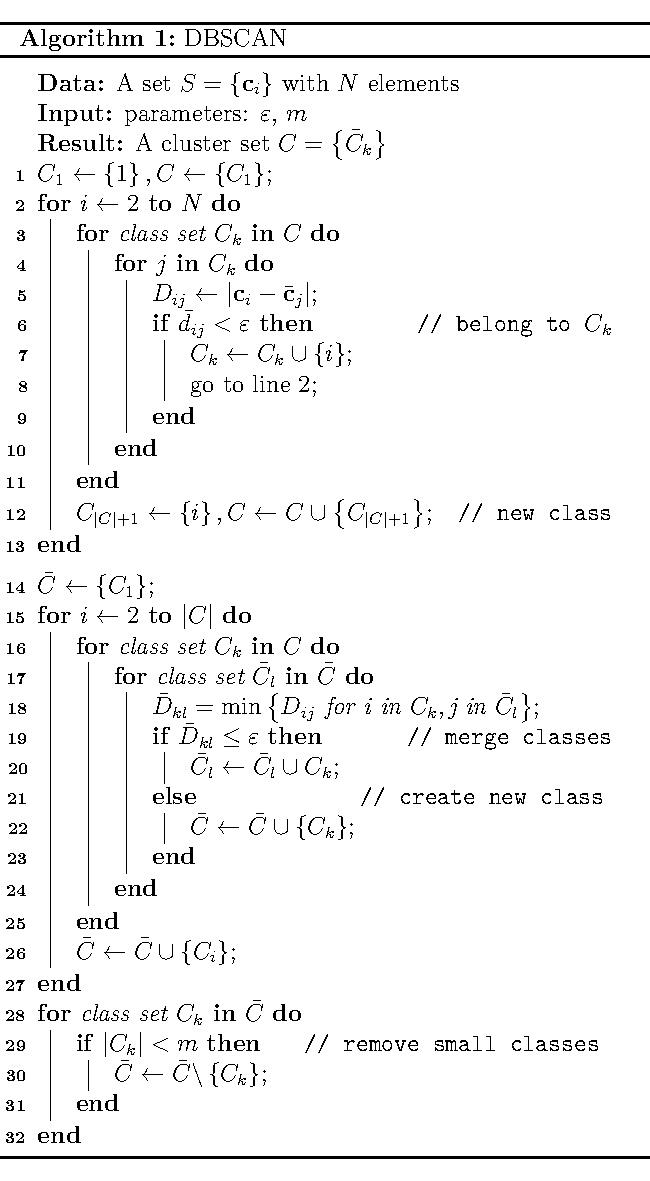
\includegraphics[width=0.48\textwidth]{./algorithm/algo.pdf}\label{algo:DBSCAN}
\end{figure}

We traverse all values between $0.15$ and $0.5$ with a step length of $0.05$, and for each value of $\varepsilon$, we calculate the number of clusters of Swarm state with $m=5$ (which is $0.5\%$ of the population $N=1000$ of the system). Then we record the minimum counts of clusters in total states. 
As shown in Fig.~\ref{fig:DBSCANparam}, the mean counts of clusters converges to at $\varepsilon=0.3$. Then we set $\varepsilon$ to be $0.3$, and set $m$ to be $5$.

\begin{figure}
    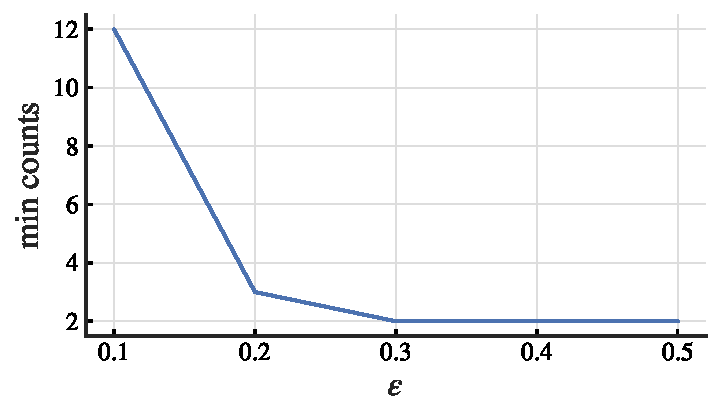
\includegraphics[width=0.48\textwidth]{./figs/DBSCANparam.pdf}
    \caption{
        \label{fig:DBSCANparam} The minimum counts of clusters with $m=0$ and different $\varepsilon$. The number of clusters is calculated by DBSCAN algorithm. 
    }
\end{figure}

% \section{\label{sec:Adiabatic} ADIABATIC TUNING OF THE ACTION RADIUS}

% \begin{figure}
%     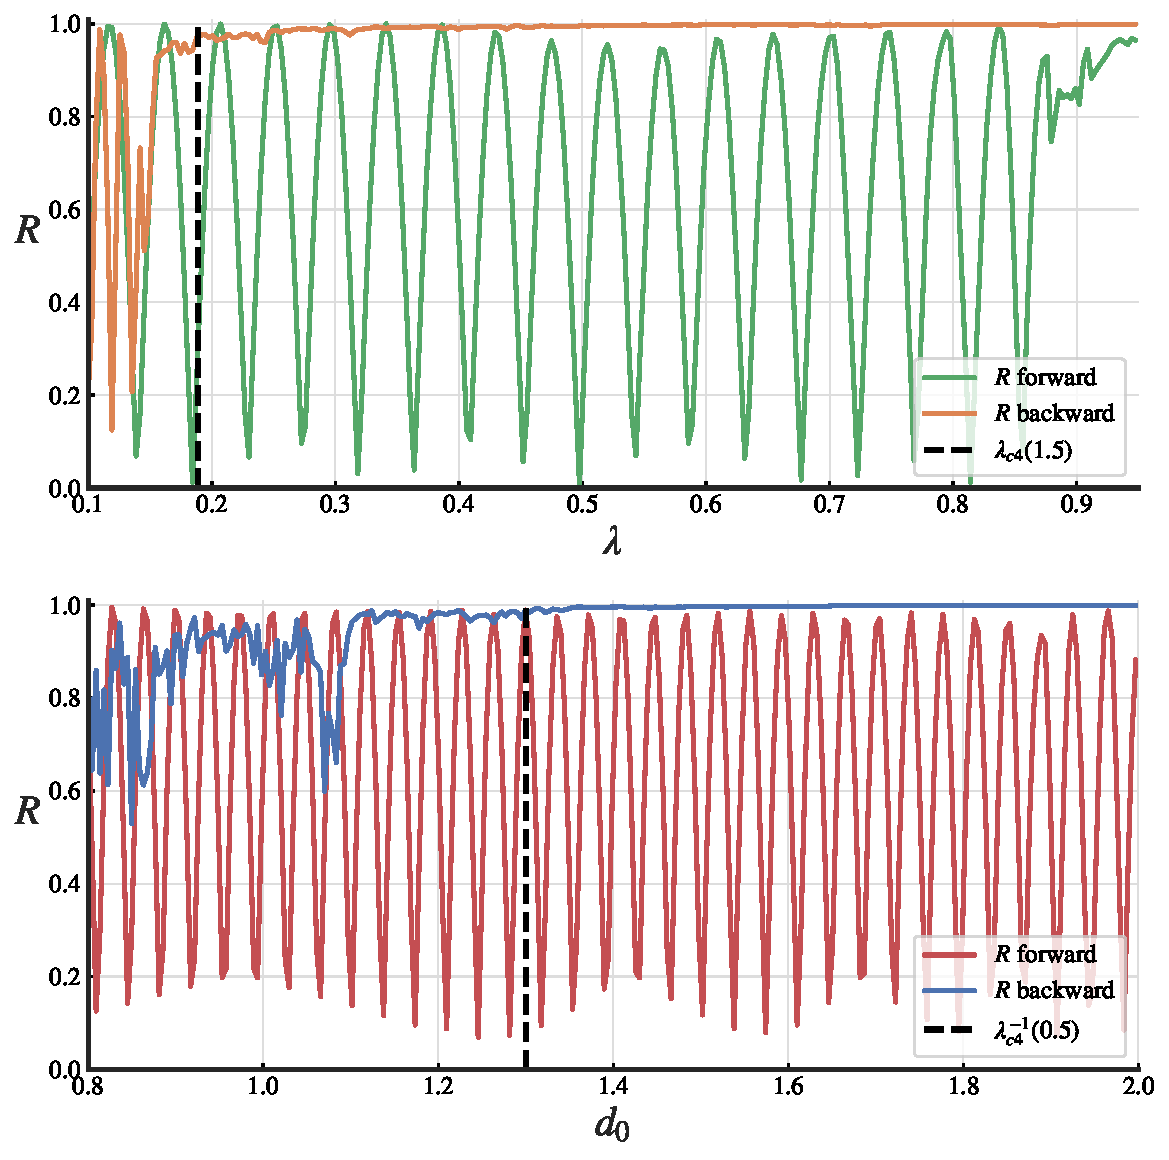
\includegraphics[width=0.48\textwidth]{./figs/aditionalTuning.pdf}
%     \caption{
%         \label{fig:adiabaticTuning} The adiabatic tuning of the coupling strength $\lambda$ and the action radius $d_0$.
%         \textbf{(a)}, The coupling strength $\lambda$ is adiabatically tuned from $0.01$ to $0.95$ with fixed $d_0=1.5$.
%         \textbf{(b)}, The action radius $d_0$ is adiabatically tuned from $0.8$ to $2$ with fixed $\lambda=0.5$.
%     }
% \end{figure}

\section{\label{sec:maxRadius} PROOF OF THE MAXIMUM RADIUS OF CLUSTERS}

In this section, we prove the maximum radius of cluster in the Swarm state is $r_c$, which is the radius of its rotation trajectory. We prove this by contradiction method.

\begin{proof}
    We assume that the maximum radius of the cluster is $r_s>r_c$. Then we have the case that the center of cluster's rotation trajectory is inside the cluster circle with radius $r_s$. 
    Fig.~\ref{fig:rsProofEps} shows the schematic plot of this case. $A$ and $B$ 
    are the centers of the cluster and trajectory circle, respectively. The cluster circle is divided into two parts by $B$: red solid and red // hatching. In order to enable cluster to move along the trajectory, the oscillators in two parts must have contrary phase velocities. This contradicts the fact that the oscillators in the cluster are synchronized. Therefore, the maximum radius of the cluster is $r_c$.
\end{proof}

\begin{figure}
    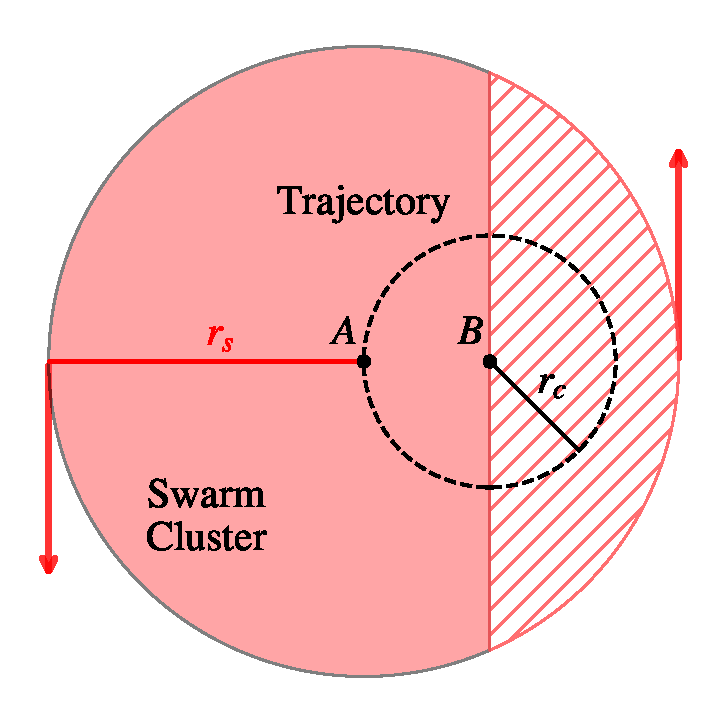
\includegraphics[width=0.25\textwidth]{./figs/rsProofEps.pdf}
    \caption{
        \label{fig:rsProofEps} The schematic plot of $r_s>r_c$.
    }
\end{figure}

\begin{figure*}
    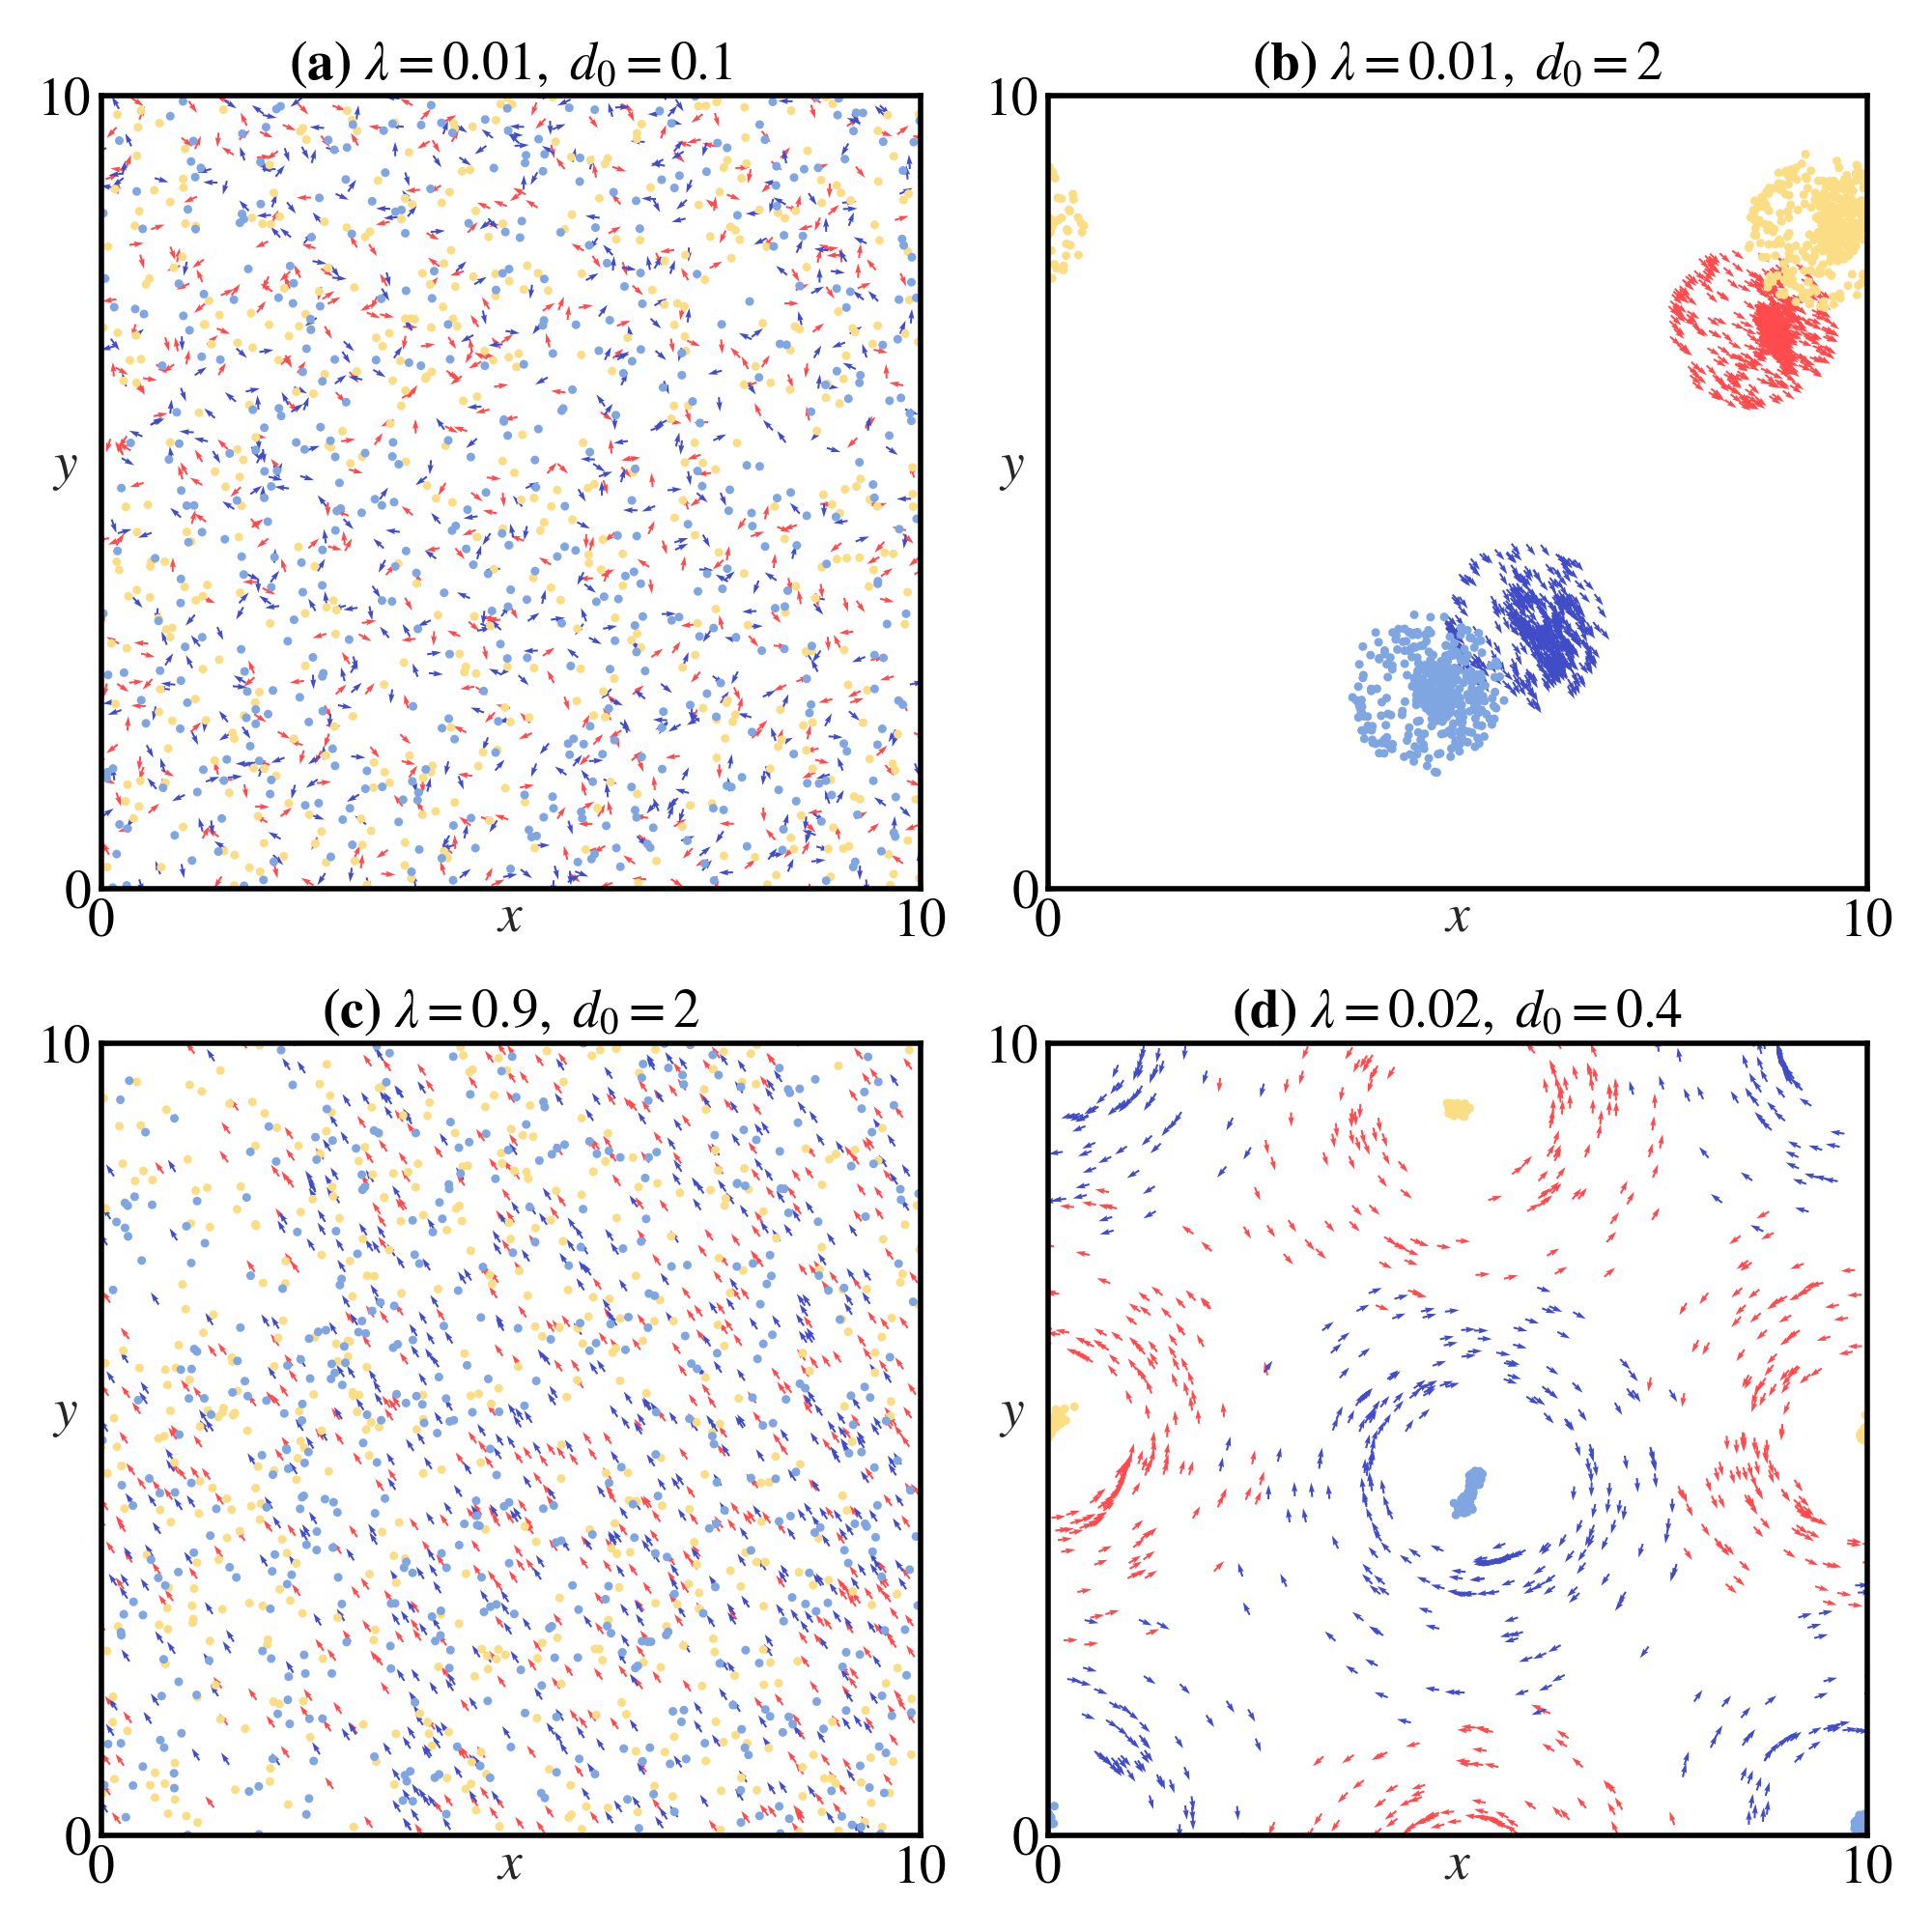
\includegraphics[width=0.7\textwidth]{./figs/etimateCenter.png}
    \caption{
        \label{fig:etimateCenter} Estimation results of real-time rotational centers. 
        The centers of two types of chirality oscillators are represented by light yellow ($\omega_i > 0$) and light blue
        ($\omega_i < 0$) points, respectively.
        \textbf{(a)}, Disorder state ($\lambda=0.01,\ d_0=0.1$).
        \textbf{(b)}, Swarm state, ($\lambda=0.01,\ d_0=2$).
        \textbf{(c)}, Quick Sync stat ($\lambda=0.9,\ d_0=2$).
        \textbf{(d)}, Ring state ($\lambda=0.02,\ d_0=0.4$).
    }
\end{figure*}

$$
$$
$$
$$
\hrulefill
\nocite{*}
\bibliography{aipsamp}

\end{document}